% Report template for EES403 Group 1, based on the IISER Mohali MS thesis template.
% Do not edit report.tex: it is generated from this file by scripts/build_latex.py,
% which fills every double-angle placeholder with a value read from results/tables.
\documentclass[a4paper, 12pt, oneside]{report}
\usepackage{geometry}
\pdfinfoomitdate=1   % no creation date in the PDF metadata
\pdftrailerid{}
\geometry{a4paper, left=1.25in, right=1in, top=1in, bottom=1in, headheight=15pt}

\usepackage{graphicx}
\usepackage{fancyhdr}
\usepackage{amsmath}
\usepackage{amssymb}
\usepackage{float}
\usepackage{titlesec}
\usepackage{mathptmx}          % Times New Roman, as in the template
\usepackage[T1]{fontenc}
\usepackage{microtype}
\usepackage{booktabs}
\usepackage{tabularx}
\usepackage{xltabular}   % tables that may break across pages
\usepackage{array}
\usepackage[table]{xcolor}
\usepackage{caption}
\usepackage{enumitem}
\usepackage[most]{tcolorbox}
\usepackage[round]{natbib}
\usepackage[hidelinks]{hyperref}
\usepackage{bookmark}

\hypersetup{pdftitle={Low-pass and High-pass Filtering of Sentinel-2 Imagery},
            pdfauthor={Group 1: Pranay Chakraborty, Sangeeta Kumari, Aparna Manoj, Robin, Sangam}, pdfsubject={EES403 Advanced Remote Sensing and GIS}}

\graphicspath{{figures/}{../../results/figures/}{../../results/figures/slides/}{../../docs/}}
\linespread{1.3}
\setlist{itemsep=2pt, topsep=4pt}
\captionsetup{font=small, labelfont=bf, margin=10pt}
\renewcommand{\arraystretch}{1.15}
% Let figures and tables share pages with text instead of floating to nearly empty pages.
\renewcommand{\topfraction}{0.9}
\renewcommand{\bottomfraction}{0.8}
\renewcommand{\textfraction}{0.07}
\renewcommand{\floatpagefraction}{0.75}
\setcounter{totalnumber}{4}
\definecolor{accent}{HTML}{1F5A96}
\definecolor{boxbg}{HTML}{EEF3F9}

% Running header: chapter name on the left, page number on the right.
\pagestyle{fancy}
\fancyhf{}
\fancyhead[L]{\small\nouppercase{\leftmark}}
\fancyhead[R]{\small\thepage}
\renewcommand{\headrulewidth}{0.4pt}
\fancypagestyle{plain}{\fancyhf{}\fancyfoot[C]{\small\thepage}\renewcommand{\headrulewidth}{0pt}}

% Short "key point" box used at the end of each results section.
\newtcolorbox{keypoint}{colback=boxbg, colframe=accent, boxrule=0.6pt, arc=2pt,
  left=6pt, right=6pt, top=4pt, bottom=4pt, fontupper=\small}
\newcommand{\fname}[1]{\textit{#1}}

% Figure and equation numbers restart in every chapter (as in the template).
\counterwithin{figure}{chapter}
\counterwithin{table}{chapter}
\counterwithin{equation}{chapter}

\begin{document}

% ---------------------------------------------------------------- title page
\thispagestyle{empty}
\newgeometry{top=1.2in, left=1.25in, right=1in, bottom=1in}
\begin{titlepage}
\begin{center}
    \LARGE
    \textbf{Low-pass and High-pass Filtering of\\Sentinel-2 Imagery over the Aravalli Ridge,\\Gurugram--Faridabad}

    \vspace{0.5cm}
    \large
    Which filtering technique suits which remote sensing application?

    \vspace{1cm}
    \Large
    \textbf{Group 1}

    \vspace{0.4cm}
    \normalsize
    \begin{tabular}{ll}
    Pranay Chakraborty & MS22041 \\
    Sangeeta Kumari & PH25084 \\
    Aparna Manoj & MS24070 \\
    Robin & MS23138 \\
    Sangam & MS23222 \\
    \end{tabular}

    \vspace{0.8cm}
    \large
    \textit{A course project report submitted for\\
    EES403: Advanced Remote Sensing and GIS}

    \vspace{0.5cm}
    \normalsize
    Instructors: Dr.\ Chandrakant Ojha and Dr.\ Meenakshi Devi

    \vspace{1.3cm}
    
\includegraphics[trim={5mm 5mm 5mm 5mm},clip,width=5cm]{HighResolutionLogo.jpg}

    \vspace{0.5cm}
    \large
    \textbf{Indian Institute of Science Education and Research, Mohali}
\end{center}
\end{titlepage}
\restoregeometry

\pagenumbering{roman}

% ---------------------------------------------------------------- abstract
\addcontentsline{toc}{chapter}{Abstract}
\begin{center}
    \textbf{\Large Abstract}
\end{center}

Filtering changes the brightness of each pixel according to the pixels around it. Low-pass filters smooth an image and high-pass filters keep only its edges, and remote sensing textbooks recommend both. We asked which of them is more useful, and for which job. We wrote <<n_filters>> filter configurations in Python, in the spatial domain (kernel convolution) and in the frequency domain (Fourier transform with masks), and applied them to one Sentinel-2 Level-2A scene of the Aravalli ridge between Gurugram and Faridabad (<<acq_date>>). Five measurable tests followed: noise removal, land-cover classification against ESA WorldCover, edge and lineament enhancement, change to the spectra, and run time.

No single filter won. A 3$\times$3 median filter removed impulse noise best (<<e1_sp_best_psnr>> dB against <<e1_sp_noisy>> dB for the noisy image). A light Gaussian low-pass raised Random Forest classification kappa from <<e2_raw_kappa>> to <<e2_best_kappa>> and halved the speckle in the map. High-pass filters lowered classification accuracy but gave the sharpest images, the best match between detected edges and mapped land-cover boundaries, and, for gradient operators, the clearest ridge lineaments. The ideal frequency mask produced ringing of <<ring_ideal>>\% at edges and should be avoided. We therefore recommend light low-pass filtering for quantitative work and high-pass products, kept as separate layers, for interpretation and structural mapping.

\newpage
\tableofcontents
\clearpage
\addcontentsline{toc}{chapter}{List of Figures}
\listoffigures
\clearpage
\addcontentsline{toc}{chapter}{List of Tables}
\listoftables
\clearpage

% ---------------------------------------------------------------- abbreviations
\chapter*{Abbreviations}
\addcontentsline{toc}{chapter}{Abbreviations}
\begin{tabular}{@{}p{2.2cm}l@{}}
AOT & Aerosol optical thickness (haze) \\
DN & Digital number, the raw value stored in a pixel \\
FFT & Fast Fourier transform \\
HPF & High-pass filter \\
LPF & Low-pass filter \\
NDVI & Normalised difference vegetation index, (NIR $-$ red)/(NIR $+$ red) \\
NIR & Near-infrared (Sentinel-2 band B8) \\
PSNR & Peak signal-to-noise ratio \\
RF & Random Forest classifier \\
SAM & Spectral angle (between two spectra) \\
SSIM & Structural similarity index \\
$D_0$ & Cutoff of a frequency mask, as a fraction of the Nyquist frequency \\
$\kappa$ & Cohen's kappa (classification agreement beyond chance) \\
$\sigma$ & Width of a Gaussian filter, in pixels \\
\end{tabular}

\medskip
Plain-language definitions of every evaluation measure are in Appendix~\ref{app:glossary}.
\clearpage

\pagenumbering{arabic}

% ================================================================ chapter 1
\chapter{Introduction}\label{chap:intro}

\section{Spatial frequency}

A satellite image is a grid of numbers. In one part of the image the numbers may stay almost the same from pixel to pixel; in another they may jump up and down every few pixels. \emph{Spatial frequency} is the number of changes in brightness (digital number, DN) per unit distance \citep{lillesand2015}. A ploughed field or a lake has low spatial frequency: grey values change gradually. A street grid, a ridge crest or a field boundary has high spatial frequency: grey values change abruptly.

Any image can be split into a low-frequency part (the broad pattern) and a high-frequency part (edges, lines, texture and noise). Spatial filters let us keep one part and suppress the other.

\section{Low-pass and high-pass filters}

A \textbf{low-pass filter (LPF)} keeps the low frequencies and removes the high ones. In practice it replaces each pixel by an average of its neighbours, so the image becomes smoother. Noise falls, but so does the sharpness of real edges.

A \textbf{high-pass filter (HPF)} does the reverse: it removes the broad pattern and keeps the abrupt changes. The classic remote sensing form is the original image minus a low-passed copy of it \citep{lillesand2015}. Uniform areas become zero (mid-grey) and only edges remain. Adding a fraction of this edge layer back to the original gives a \textbf{high-boost} or edge-enhanced image, which looks sharper but keeps its colours.

Figure~\ref{fig:profile} shows both effects on real data. Along one line across the ridge, the low-pass curves (blue) are flatter than the original (black), while the high-boost curves (pink) are steeper and overshoot at every edge.

\begin{figure}[htbp]
    \centering
    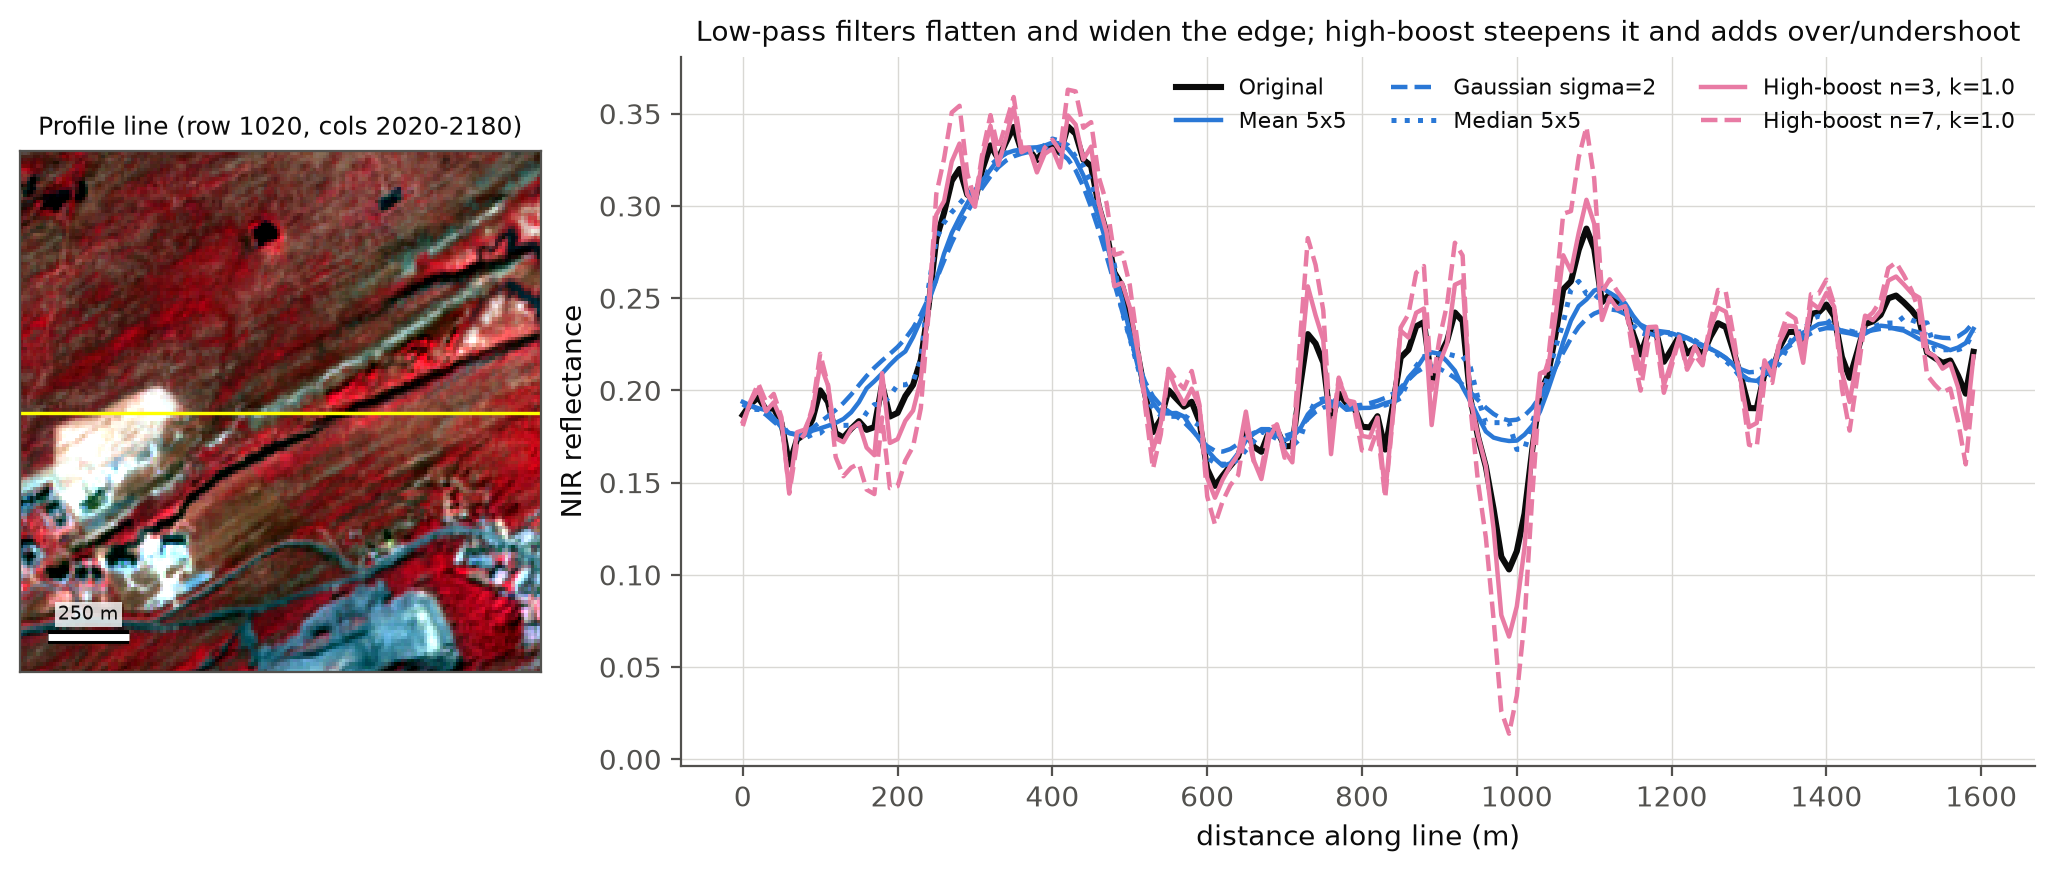
\includegraphics[width=\textwidth]{fig06_line_profile.png}
    \caption[Effect of low-pass and high-boost filters on a line profile]{Near-infrared (NIR) reflectance along a 1.6 km line across a bright cleared patch on the ridge (yellow line, left). Low-pass filters flatten and widen each edge; high-boost filters steepen it and add overshoot.}
    \label{fig:profile}
\end{figure}

Both kinds of filter can be computed in two ways. In the \emph{spatial domain} a small grid of weights (a kernel) slides over the image. In the \emph{frequency domain} the image is transformed with the fast Fourier transform (FFT), the unwanted frequencies are multiplied by zero with a mask, and the result is transformed back \citep{gonzalez2018}. Both routes appear in the course material, so we implemented both.

\section{Aim}

The project brief asked us to implement low-pass and high-pass filtering on remote sensing data and decide which technique is most suitable. Since smoothing and edge enhancement are meant for different jobs, we split the question by application:

\begin{enumerate}
    \item Which filter removes noise best?
    \item Which filter helps an automatic land-cover classification most?
    \item Which filter makes edges, boundaries and geological lineaments easiest to see?
    \item How much does each filter change the reflectance values that later analysis relies on?
    \item Is the spatial or the frequency route faster?
\end{enumerate}

Each question became one experiment (E1 to E5), and the answers were combined in a decision matrix (Chapter~\ref{chap:discussion}).

\section{How this report is organised}

Chapter~\ref{chap:data} describes the study area and the satellite data. Chapter~\ref{chap:methods} explains the filters and the five experiments. Chapter~\ref{chap:results} shows what the filters do and what each experiment found; every results section ends with a shaded box that states the main finding in one or two sentences. Chapter~\ref{chap:discussion} brings the findings together in a decision matrix and a recommendation, and Chapter~\ref{chap:summary} sums up. Appendix~\ref{app:glossary} explains each evaluation measure in plain words, Appendix~\ref{app:code} shows where each step lives in the code, and Appendix~\ref{app:repro} lists the commands that rebuild every result.

% ================================================================ chapter 2
\chapter{Study Area and Data}\label{chap:data}

\section{Study area}

The study area is a 25 km $\times$ 23 km box over the Aravalli ridge between Gurugram and Faridabad in Haryana (77.05--77.30\,$^\circ$E, 28.30--28.50\,$^\circ$N; Figure~\ref{fig:aoi}). We chose it because it holds very different textures in one scene:

\begin{itemize}
    \item folded quartzite ridges with long, parallel linear features (high frequency, useful for testing HPF);
    \item the dense street grid of Gurugram (sharp man-made edges);
    \item small crop parcels in the south-east (smooth surfaces, useful for testing LPF);
    \item old quarries and a few ponds.
\end{itemize}

Three 2 km windows (ridge, urban, cropland; yellow boxes in Figure~\ref{fig:aoi}) are used for the zoomed comparisons in Chapter~\ref{chap:results}.

\begin{figure}[htbp]
    \centering
    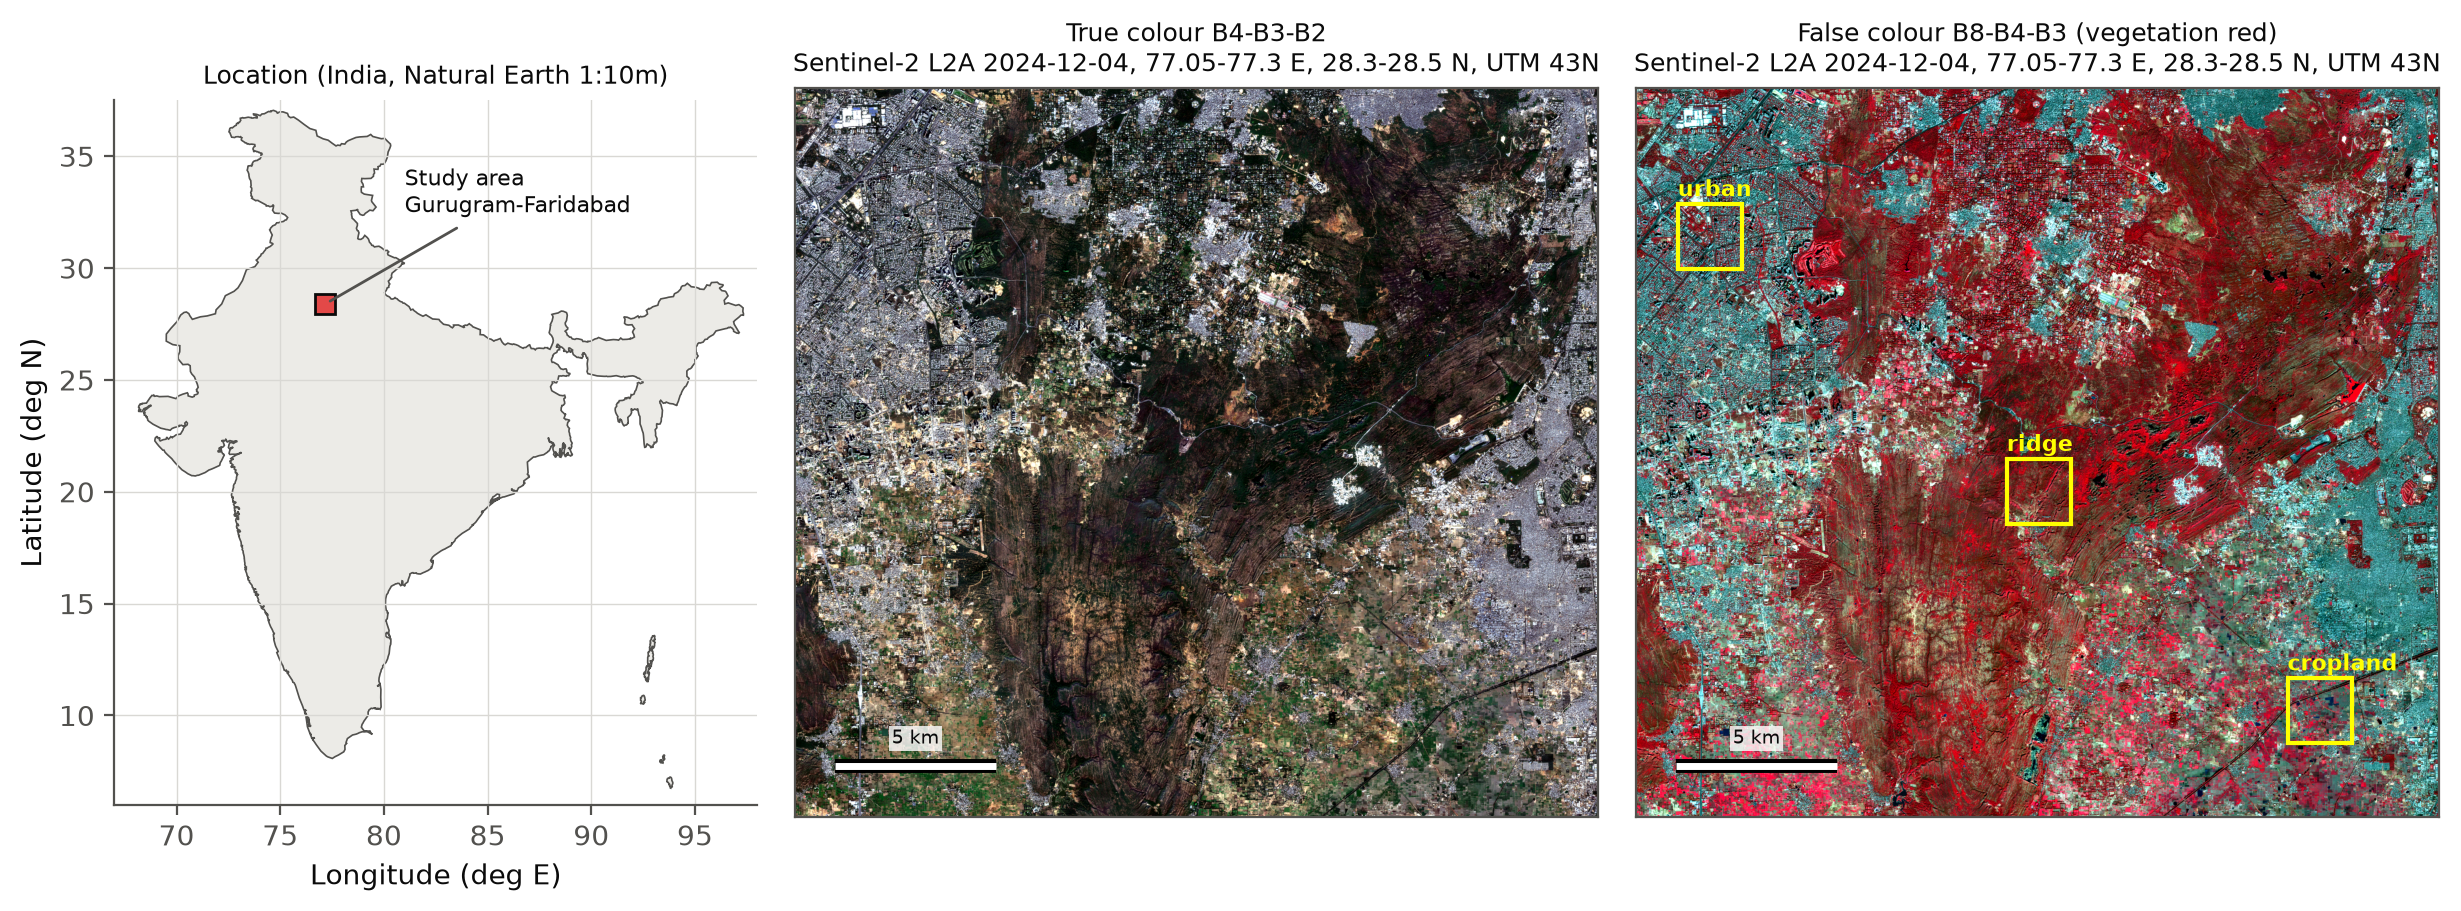
\includegraphics[width=\textwidth]{fig01_study_area.png}
    \caption[Study area and the selected Sentinel-2 scene]{Location of the study area and the selected Sentinel-2 scene in true colour (red, green, blue) and false colour (NIR, red, green; vegetation appears red). Yellow boxes mark the ridge, urban and cropland windows.}
    \label{fig:aoi}
\end{figure}

\section{Satellite data and scene selection}

We used Sentinel-2 Level-2A surface reflectance \citep{drusch2012, esa_l2a}, downloaded from Google Earth Engine. The four 10 m bands were used: blue (B2), green (B3), red (B4) and near-infrared (B8).

Winter is usually the clearest season over Delhi NCR, so the program searched 1 November 2024 to 28 February 2025 for scenes with less than 5\% cloud. <<n_candidates>> scenes qualified. Scene-wide cloud cover turned out to be a poor guide: inside our box the share of cloudy, hazy or missing pixels ranged from <<bad_min>>\% to <<bad_max>>\%, because winter smog does not count as cloud in the scene-wide figure. The program therefore scored every candidate inside the study area only, using the Sentinel-2 scene classification layer, the s2cloudless cloud probability and the aerosol optical thickness (AOT), and picked the cleanest, least hazy scene.

\begin{table}[htbp]
\centering
\caption{Scene and data summary.}
\label{tab:data}
\small
\begin{tabularx}{\textwidth}{@{}lX@{}}
\toprule
Item & Value \\
\midrule
Product & {\scriptsize\texttt{<<product_id>>}} \\
Acquisition & <<acq_date>>, <<acq_time>> UTC; tile <<tile>>; processing baseline <<baseline>> \\
Flagged pixels in the study area & <<bad_pct>>\% (cloud, cirrus, shadow, no data or haze); mean AOT <<aot>> \\
Bands & B2, B3, B4, B8 at 10 m \\
Grid & <<width>> $\times$ <<height>> pixels, UTM zone 43N (EPSG:32643), aligned to the native pixels \\
Reflectance & DN / 10000, clipped to [0, 1] \\
Land-cover reference & ESA WorldCover 2021 v200 \citep{zanaga2022}, regridded by nearest neighbour \\
Demo subset & 512 $\times$ 512 pixel crop with the most varied land cover \\
\bottomrule
\end{tabularx}
\end{table}

\section{Land-cover reference}

ESA WorldCover 2021 \citep{zanaga2022} gives a land-cover class for every 10 m pixel. We merged its classes into six groups: Trees, Shrub/Grass, Cropland, Built-up, Bare/Mining and Water. Water covered only <<water_pct>>\% of the area and was dropped, which left five classes: Trees (<<cls_trees>>\%), Shrub/Grass (<<cls_shrub>>\%), Cropland (<<cls_cropland>>\%), Built-up (<<cls_built>>\%) and Bare/Mining (<<cls_bare>>\%). WorldCover is itself produced by a classifier, so it is a reference map, not ground truth.

% ================================================================ chapter 3
\chapter{Methods}\label{chap:methods}

\section{Workflow}

Figure~\ref{fig:flow} shows the processing chain. Every step is a Python function in the package \texttt{rsfilter}; one command (\texttt{python scripts/run\_all.py}) repeats the whole analysis, and the random seed is fixed at 42.

\begin{figure}[htbp]
    \centering
    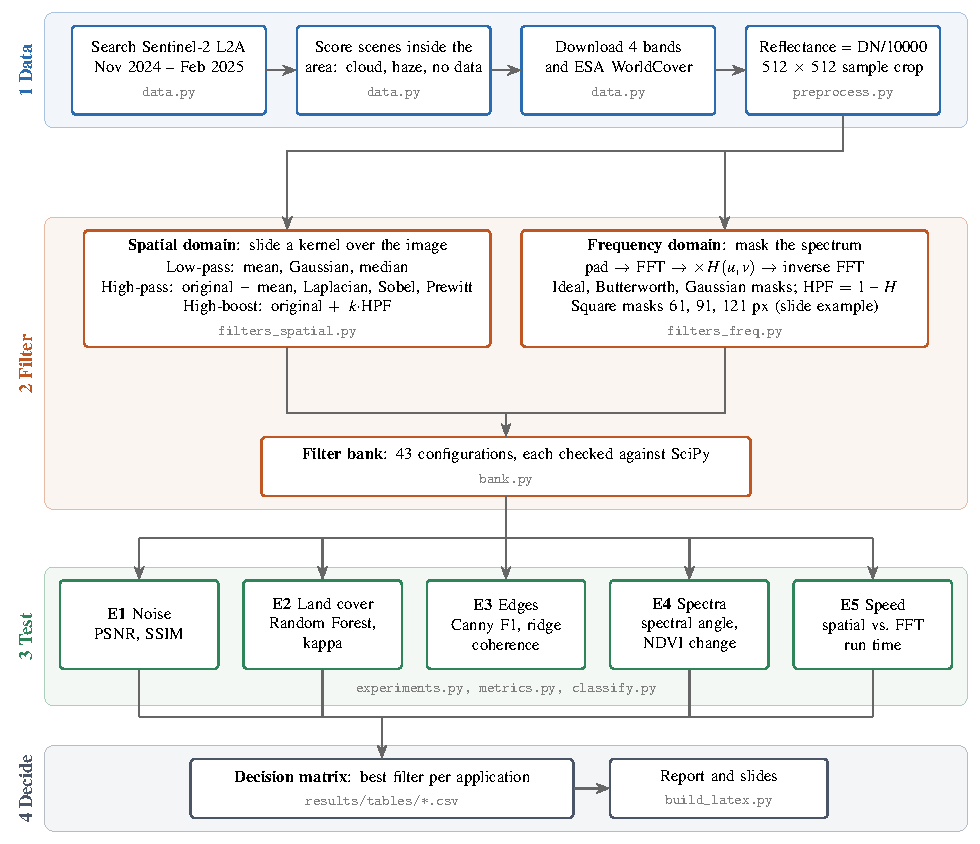
\includegraphics[width=\textwidth]{flowchart.pdf}
    \caption[Processing flowchart]{Processing flowchart. The work runs in four stages, top to bottom; the grey text in each box names the Python module that does the step (Appendix~\ref{app:code}).}
    \label{fig:flow}
\end{figure}

All filters were written in NumPy. Unit tests compare them with the reference library \texttt{scipy.ndimage}; the largest difference is below $10^{-5}$. Each filter works band by band on float32 reflectance. At the image border the image is mirrored, so no artificial black frame enters the result.

\section{Spatial-domain filters}

A spatial filter computes each output pixel $g(x,y)$ as a weighted sum of the input pixels $f$ around it, with the weights held in a kernel $w$ of size $(2a+1)\times(2b+1)$:
\begin{equation}
    g(x,y) = \sum_{s=-a}^{a}\sum_{t=-b}^{b} w(s,t)\, f(x-s,\, y-t).
    \label{eq:conv}
\end{equation}
This is convolution; it turns the kernel by 180$^\circ$, which makes no difference for the symmetric kernels used here. Instead of looping over pixels, our code loops over the few kernel cells: for each cell it shifts the whole padded image by $(s,t)$, multiplies it by $w(s,t)$ and adds it to the output. This uses little memory and is easy to check.

\paragraph{Low-pass kernels.} The \emph{mean} filter uses equal weights, for example
\begin{equation}
    w_{\text{mean},3} = \frac{1}{9}\begin{bmatrix}1&1&1\\1&1&1\\1&1&1\end{bmatrix}.
\end{equation}
The \emph{Gaussian} filter gives nearby pixels more weight, $w(s,t) \propto \exp\!\big(-(s^2+t^2)/2\sigma^2\big)$, with a kernel side of $2\lceil 3\sigma\rceil+1$ and weights that sum to 1. The \emph{median} filter is not a weighted sum: it replaces each pixel by the median of its neighbourhood, which ignores single extreme values.

\paragraph{High-pass kernels.} The remote sensing HPF subtracts a mean filter from the image \citep{lillesand2015}:
\begin{equation}
    \text{HPF}_n = f - \text{mean}_{n\times n}(f).
\end{equation}
The Laplacian responds to a change in slope in any direction, and the Sobel and Prewitt operators measure the gradient in $x$ and $y$; we use the gradient magnitude $\sqrt{G_x^2+G_y^2}$:
\begin{equation}
    w_{\text{Lap},4} = \begin{bmatrix}0&1&0\\1&-4&1\\0&1&0\end{bmatrix},\qquad
    w_{\text{Sobel},x} = \begin{bmatrix}-1&0&1\\-2&0&2\\-1&0&1\end{bmatrix},\qquad
    w_{\text{Prewitt},x} = \begin{bmatrix}-1&0&1\\-1&0&1\\-1&0&1\end{bmatrix}.
\end{equation}
The 8-neighbour Laplacian also uses the diagonals; $G_y$ uses the transposed kernel.

\paragraph{High-boost.} An analyst rarely looks at the bare edge layer. High-boost adds it back to the image with a weight $k$:
\begin{equation}
    \text{enhanced} = f + k\cdot\text{HPF}_n .
\end{equation}

\section{Frequency-domain filters}

In the frequency domain, filtering is a multiplication \citep{gonzalez2018}:
\begin{equation}
    g = \mathcal{F}^{-1}\big\{ H(u,v)\cdot \mathcal{F}\{f\} \big\},
    \label{eq:fft}
\end{equation}
where $\mathcal{F}$ is the 2-D FFT and $H$ is a mask that is 1 for frequencies we keep and 0 (or close to 0) for those we remove. Our pipeline per band is: mirror-pad by 64 pixels, FFT, shift the zero frequency to the centre, multiply by $H$, shift back, inverse FFT, keep the real part, and crop the padding. The padding matters: the FFT treats the image as if it repeated forever, so without padding the left border would leak into the right border.

Let $D$ be the distance from the centre of the spectrum, scaled so that $D=1$ at the Nyquist frequency (the highest frequency a 10 m grid can hold), and $D_0$ the cutoff. We used three low-pass masks:
\begin{align}
    \text{Ideal:}\quad & H = 1 \text{ if } D \le D_0, \text{ else } 0\\
    \text{Butterworth (order 2):}\quad & H = 1 / \big(1 + (D/D_0)^{4}\big)\\
    \text{Gaussian:}\quad & H = \exp\!\big(-D^2/2D_0^2\big)
\end{align}
with $D_0 = 0.1$, 0.2 and 0.3. Each high-pass mask is $1-H$. A Gaussian mask with cutoff $D_0$ is the same filter as a spatial Gaussian with $\sigma = 1/(\pi D_0)$ pixels, which gave us a direct check between the two domains. To reproduce the example in the course slides, we also applied square ideal low-pass masks of 61, 91 and 121 pixels to the 512 $\times$ 512 crop.

\begin{table}[htbp]
\centering
\caption{Filter bank: the <<n_filters>> configurations compared.}
\label{tab:bank}
\small
\begin{tabularx}{\textwidth}{@{}llX@{}}
\toprule
Family & Filter & Parameters \\
\midrule
Low-pass, spatial & Mean & $n = 3, 5, 7, 9$ \\
 & Gaussian & $\sigma = 1, 2, 3$ pixels \\
 & Median & $n = 3, 5$ \\
Low-pass, frequency & Ideal, Butterworth ($n=2$), Gaussian & $D_0 = 0.1, 0.2, 0.3$ of Nyquist \\
High-pass, spatial & Original $-$ mean & $n = 3, 5, 7$ \\
 & Laplacian & 4- and 8-neighbour \\
 & Sobel, Prewitt & gradient magnitude \\
High-pass, frequency & Ideal, Butterworth, Gaussian & $1 - H$, $D_0 = 0.1, 0.2, 0.3$ \\
High-boost & $f + k\cdot\text{HPF}_n$ & $n = 3, 5, 7$; $k = 0.5, 1.0, 1.5$ \\
\bottomrule
\end{tabularx}
\end{table}

\section{Experiments}

Table~\ref{tab:experiments} lists the five experiments. Each writes one table to \texttt{results/tables/}, and every number in this report is read from those tables by a script.

\begin{table}[htbp]
\centering
\caption{The five experiments.}
\label{tab:experiments}
\small
\begin{tabularx}{\textwidth}{@{}lXX@{}}
\toprule
 & Question and set-up & Measure \\
\midrule
E1 & Noise removal. Add Gaussian noise ($\sigma = 0.02$) or 2\% salt-and-pepper noise to the clean 512 $\times$ 512 crop, then apply each low-pass filter. & PSNR and SSIM \citep{wang2004} against the clean crop (higher is better). \\
E2 & Classification. Random Forest \citep{breiman2001}, 200 trees, 2000 training pixels per class, on the four bands plus NDVI computed after filtering. Inputs: raw bands, each LPF, each high-boost image, and raw bands with HPF layers added. & Overall accuracy, Cohen's $\kappa$, macro-F1; salt-and-pepper index = share of pixels whose class differs from most of their 3 $\times$ 3 neighbours. \\
E3 & Edges and lineaments on the NIR band. & Average gradient; F1 of Canny edges \citep{canny1986} against WorldCover class boundaries (2-pixel tolerance); orientation coherence on the ridge \citep{bigun1987}. \\
E4 & Spectral change caused by the filter. & Correlation, RMSE, spectral angle (SAM), change in NDVI. \\
E5 & Speed on one full band (<<e5_shape>> pixels). & Median of 5 runs, spatial vs.\ frequency route. \\
\bottomrule
\end{tabularx}
\end{table}

Two choices in E2 and E3 need a short explanation.

\paragraph{Blocked train/test split (E2).} Neighbouring pixels are very similar. If training and test pixels are drawn at random, almost every test pixel has a near-copy in the training set, and accuracy looks better than it is. We therefore cut the area into 128 $\times$ 128 pixel blocks and gave 70\% of the blocks to training and 30\% to testing (<<n_train_pix>> training and <<n_test_pix>> test pixels before sampling).

\paragraph{Orientation coherence (E3).} The study area has no published lineament map, so we needed a measure of how strongly linear an image is. Coherence, computed from the structure tensor in a 2 $\times$ 2 km ridge window, is 1 when all local gradients point the same way (parallel ridges) and 0 when they point in random directions (speckle).

% ================================================================ chapter 4
\chapter{Results}\label{chap:results}

\section{What the filters do to the image}

Figure~\ref{fig:lpf} shows low-pass results on the ridge and urban windows. All low-pass filters blur the street grid and field edges; the broad shape of the ridge survives. The median keeps straight edges a little sharper than a mean or Gaussian of the same size, because it picks an existing value rather than averaging across the edge. The ideal frequency mask leaves a faint ripple texture; the Gaussian frequency mask looks like the spatial Gaussian, as expected.

\begin{figure}[htbp]
    \centering
    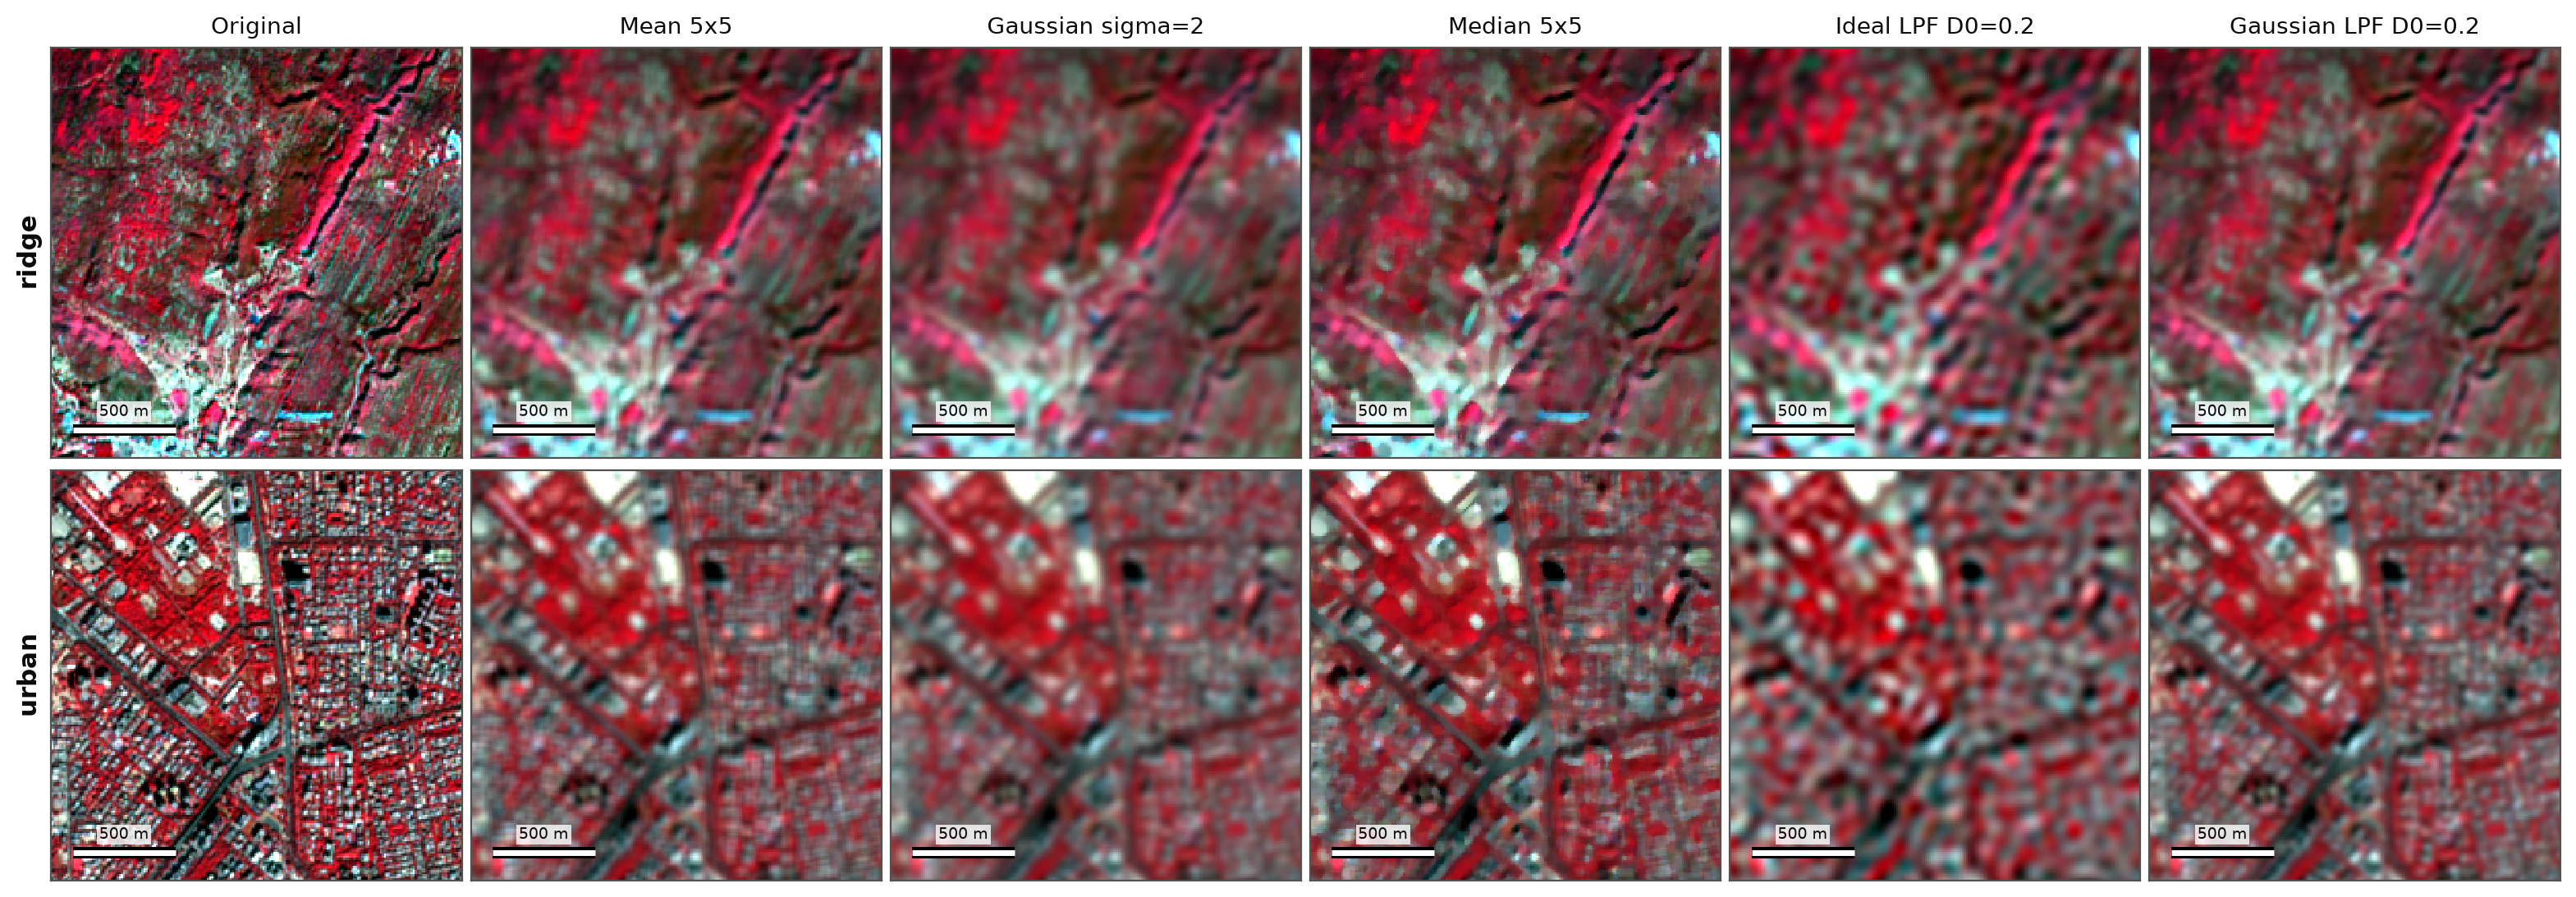
\includegraphics[width=\textwidth]{slide_lpf.png}
    \caption[Low-pass filter results]{Low-pass results on 2 km windows over the ridge (top) and Gurugram (bottom), false colour, same colour stretch in every panel.}
    \label{fig:lpf}
\end{figure}

High-pass outputs (Figure~\ref{fig:hpf}) are edge maps: flat ground turns mid-grey and only changes remain. The 7 $\times$ 7 HPF and the low-cutoff frequency HPF bring out the ridge crests. The Laplacian reacts most to fine speckle. Sobel shows edge strength without regard to direction. High-boost images (Figure~\ref{fig:boost}) keep the colours and sharpen boundaries; at $k = 1.5$ bright and dark halos appear along roads and ridge crests.

\begin{figure}[htbp]
    \centering
    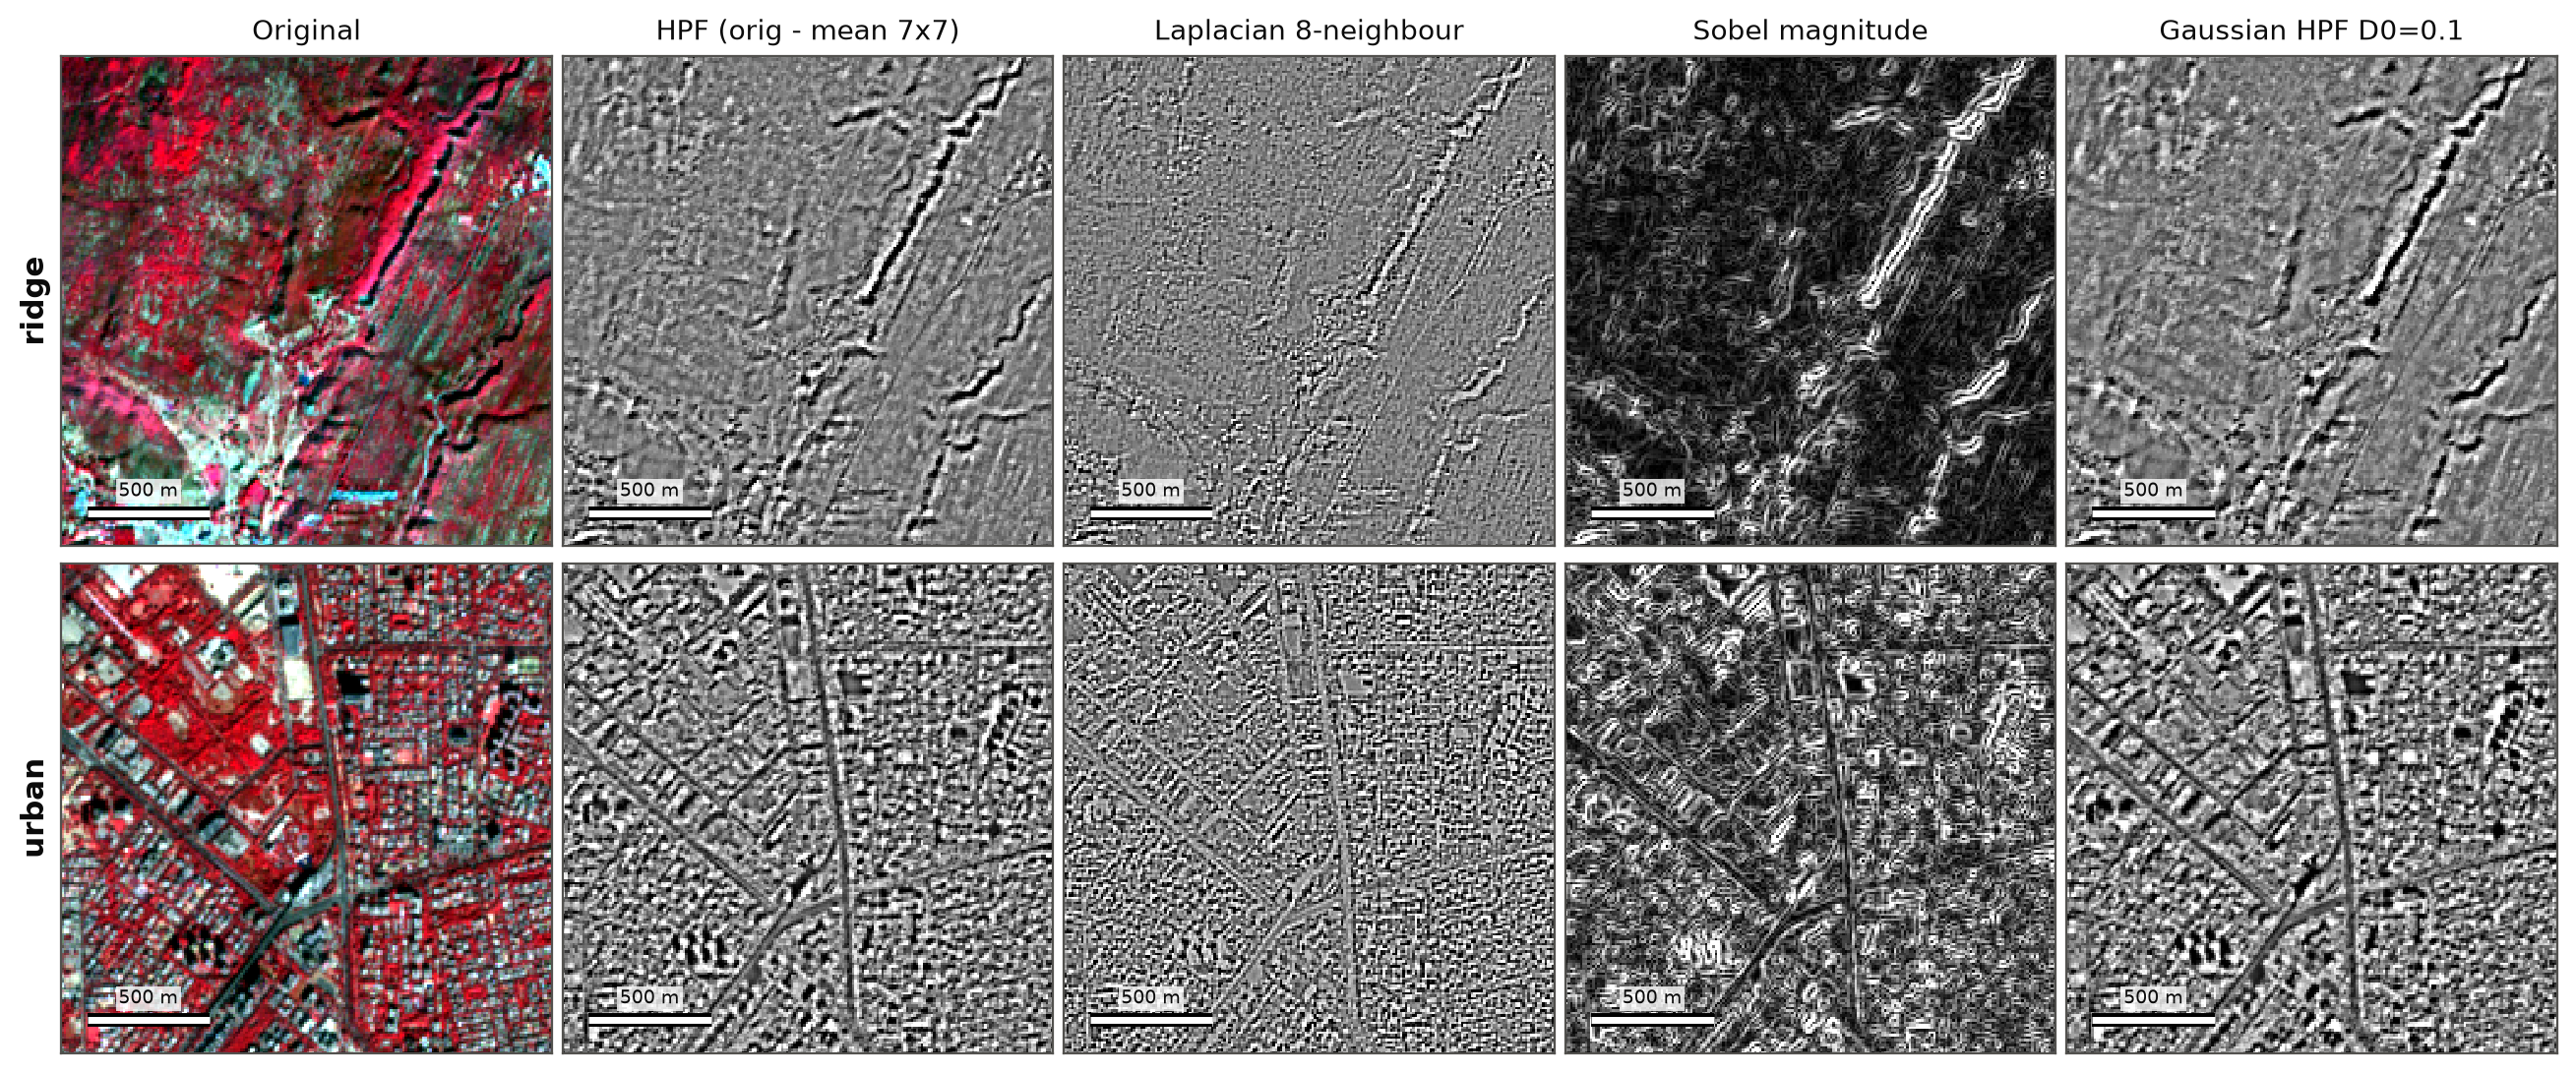
\includegraphics[width=\textwidth]{slide_hpf_edges.png}
    \caption[High-pass filter results]{High-pass results on the NIR band for the same two windows.}
    \label{fig:hpf}
\end{figure}

\begin{figure}[htbp]
    \centering
    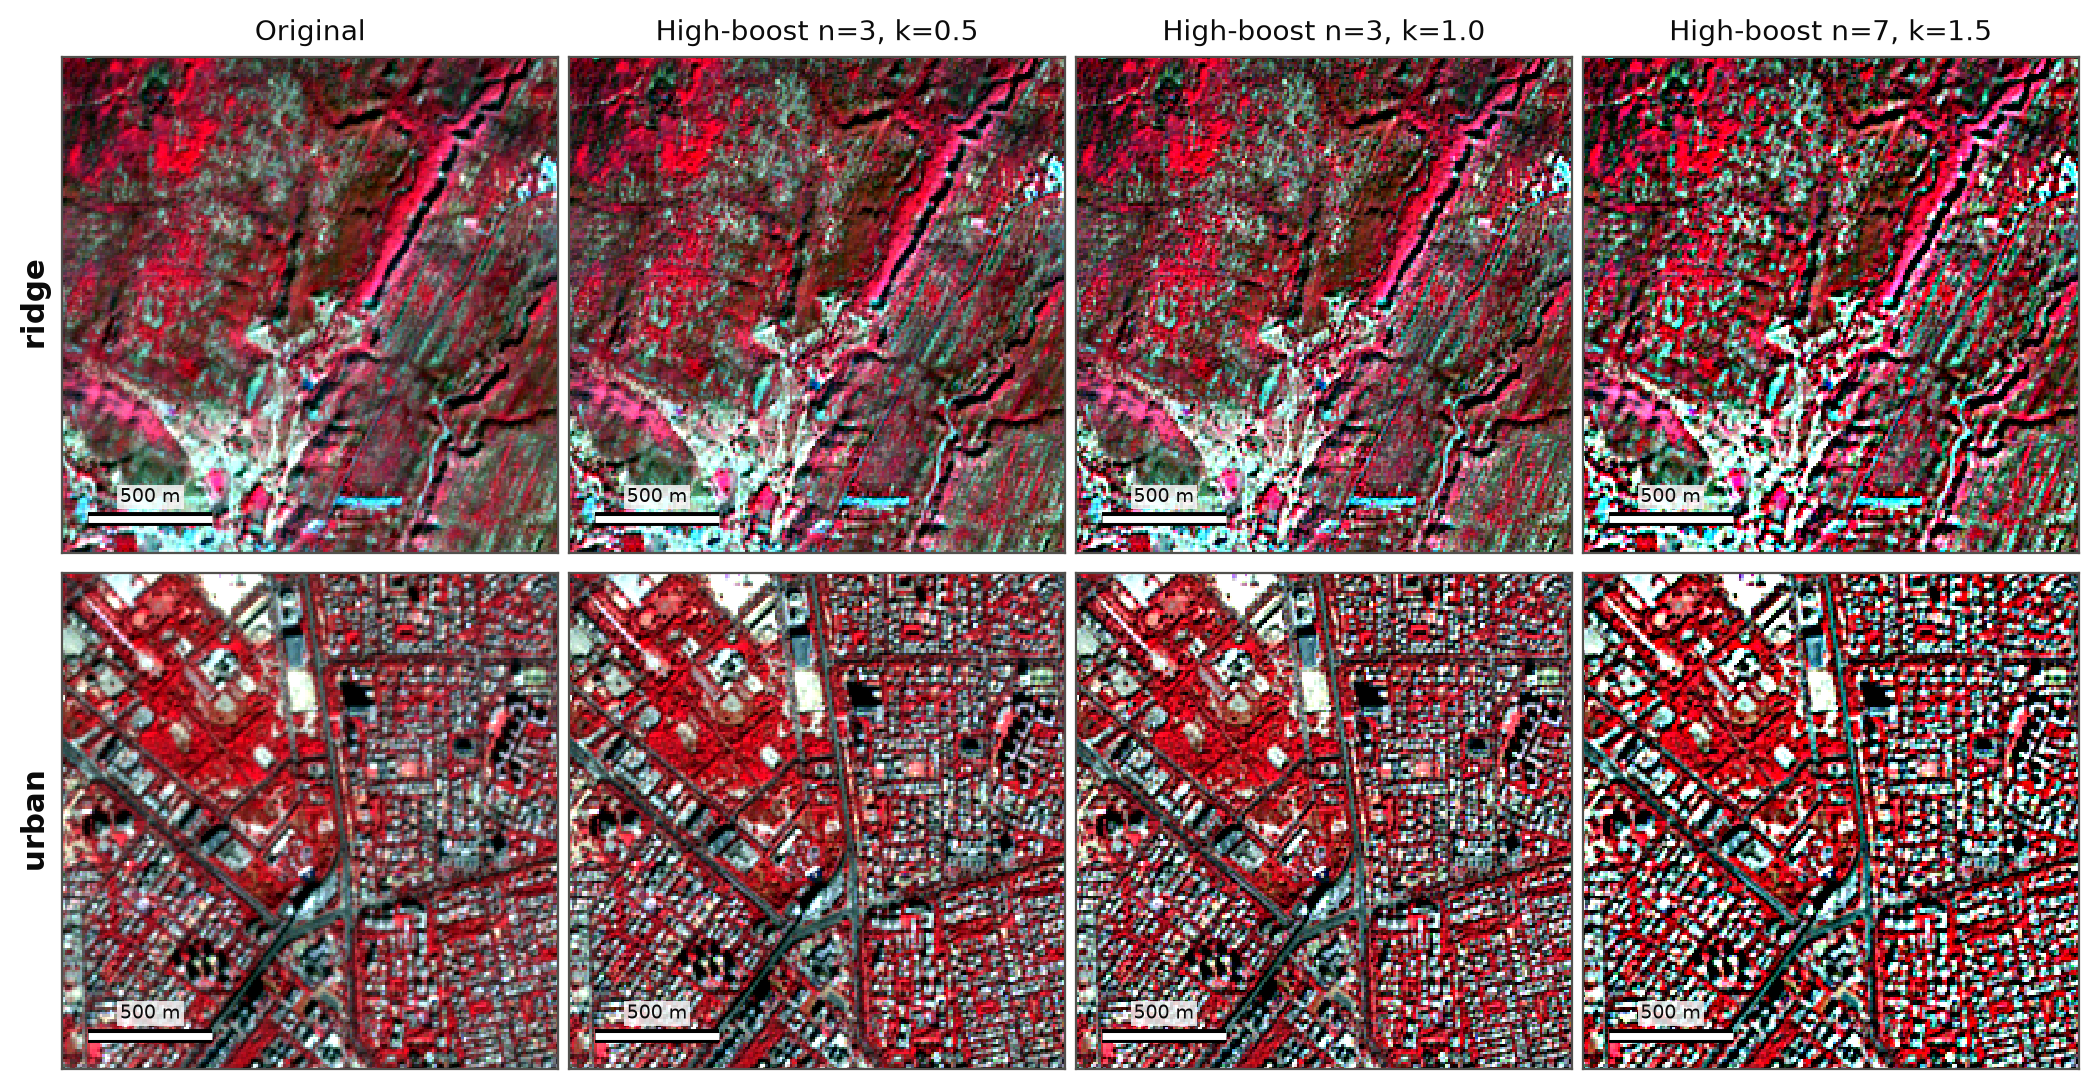
\includegraphics[width=\textwidth]{slide_highboost.png}
    \caption[High-boost results]{High-boost (original $+\,k\cdot$HPF) for increasing $k$, false colour.}
    \label{fig:boost}
\end{figure}

\section{Frequency domain and ringing}

Figure~\ref{fig:square} reproduces the course slide. The smaller the square mask, the fewer frequencies pass and the blurrier the result; all three results show a ripple texture.

\begin{figure}[htbp]
    \centering
    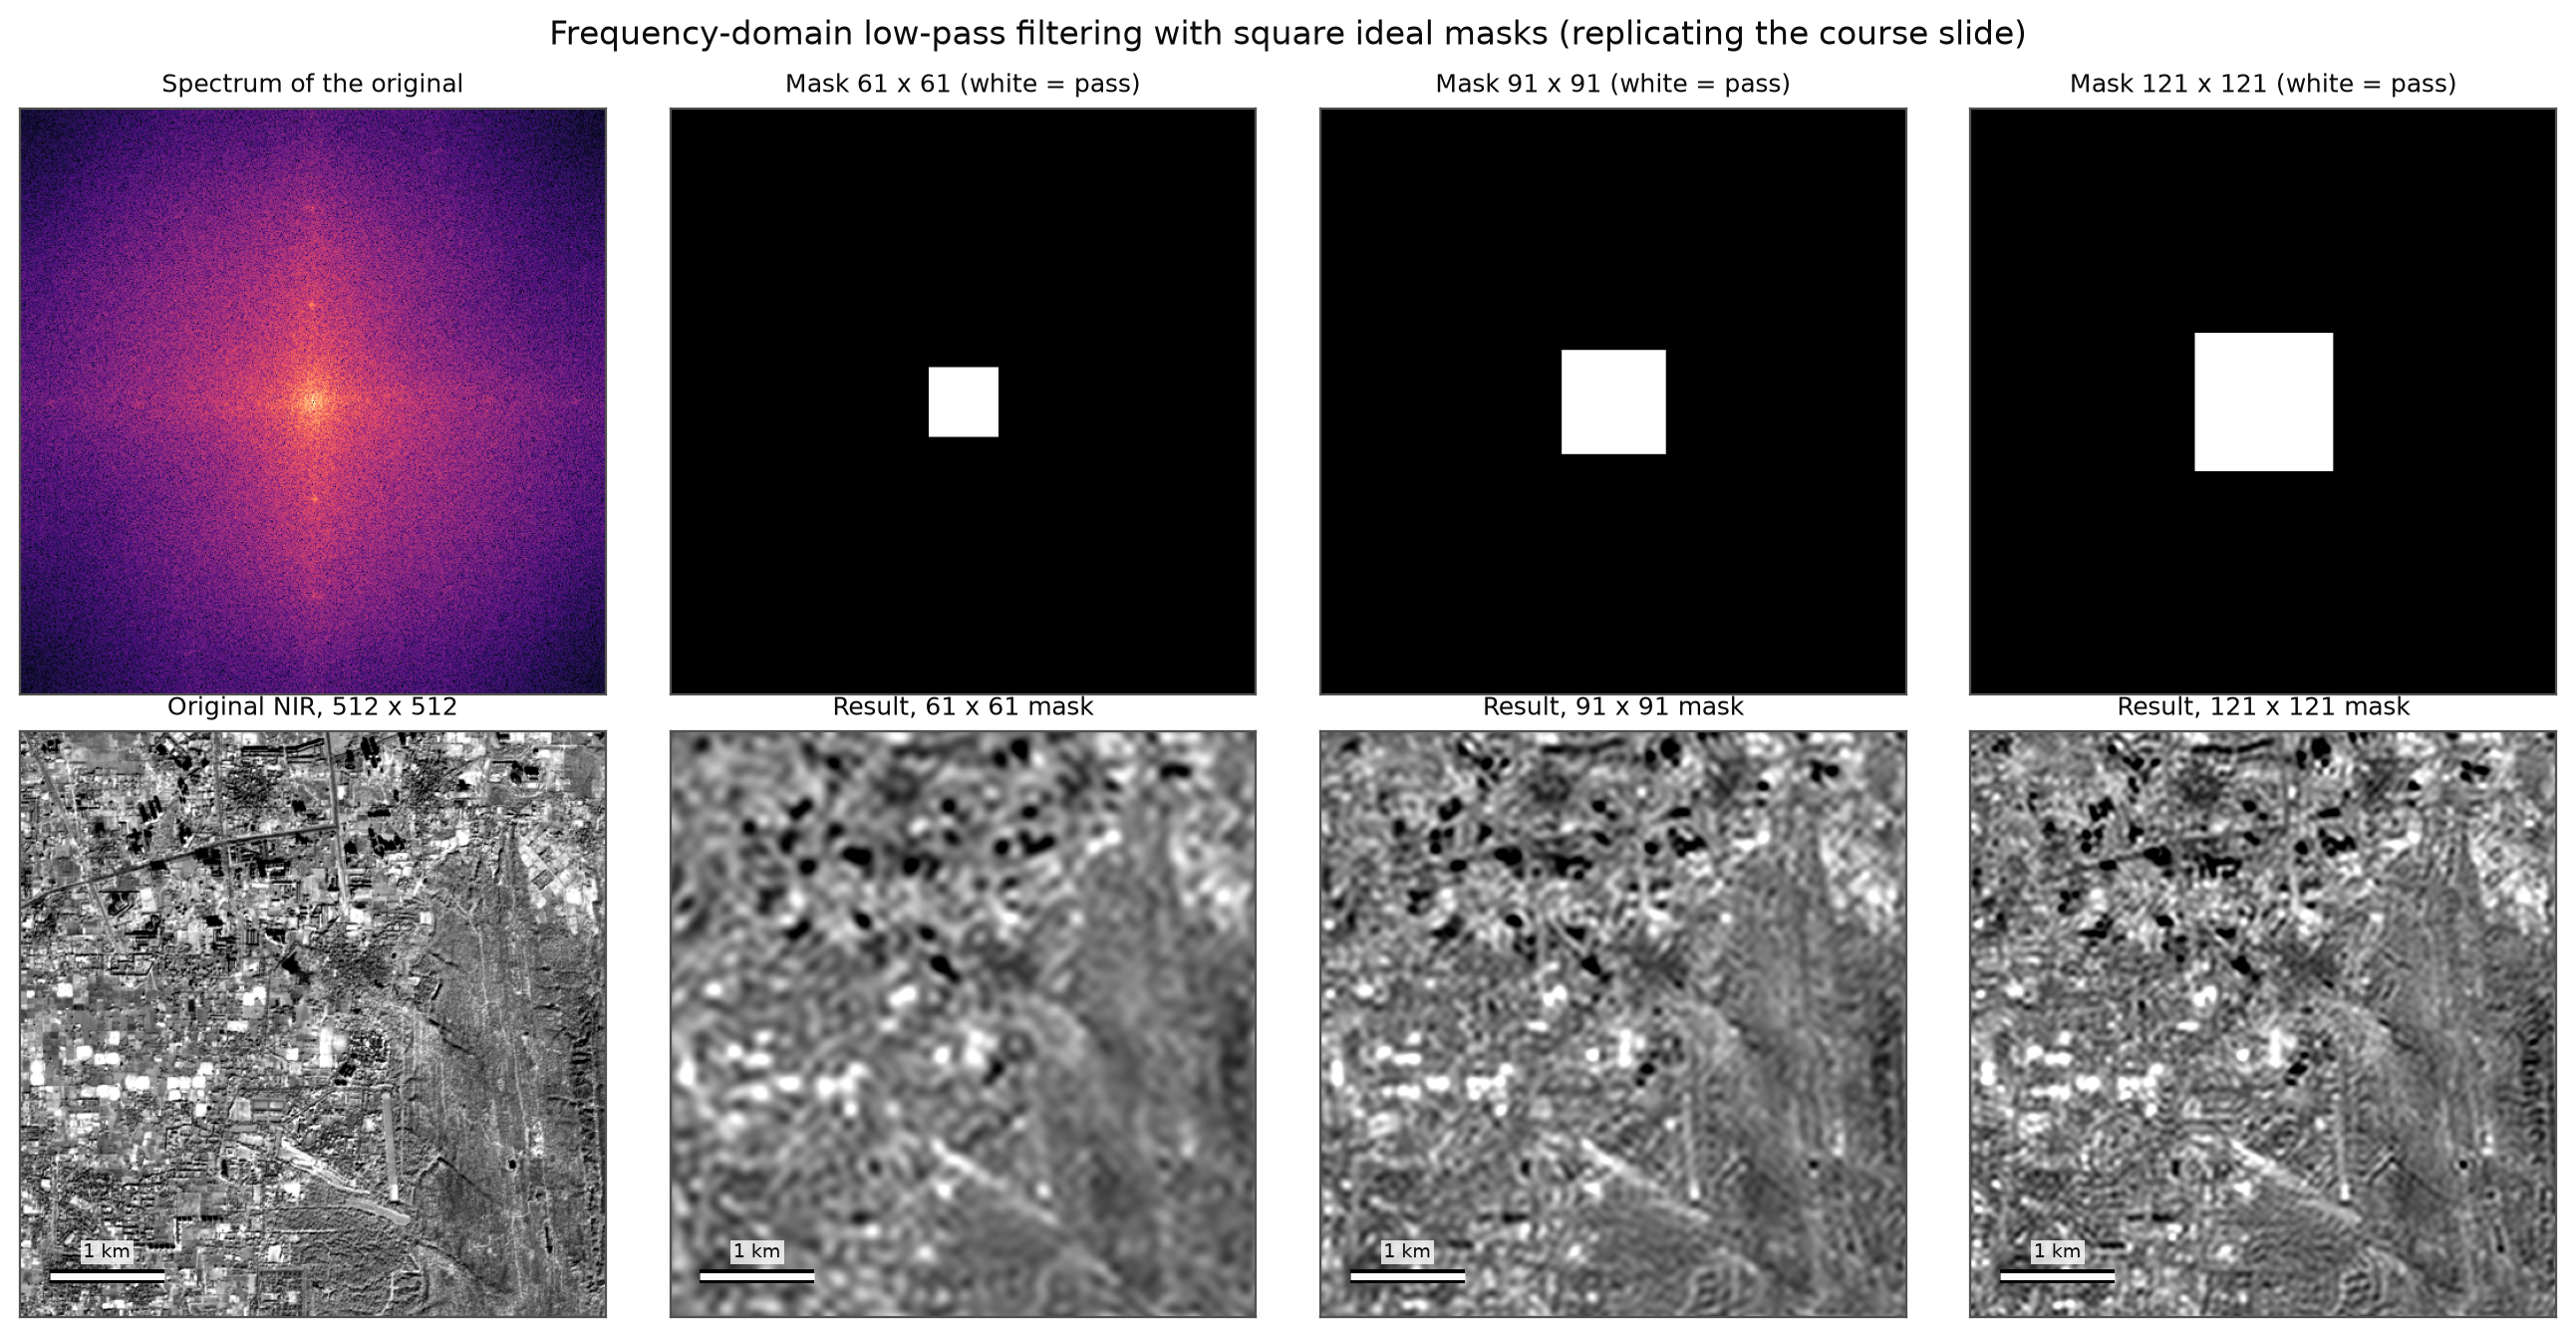
\includegraphics[width=\textwidth]{fig04_slide_square_masks.png}
    \caption[Square ideal masks of 61, 91 and 121 pixels]{Reproduction of the course slide: square ideal low-pass masks of 61, 91 and 121 pixels (top) and the filtered NIR crop (bottom).}
    \label{fig:square}
\end{figure}

These ripples are \emph{ringing}. A mask with a sharp edge in frequency produces oscillations beside every edge in the image (the Gibbs effect; \citealp{gonzalez2018}). On real data the ripples are hidden by texture, so we passed a clean step edge through the same code (Figure~\ref{fig:ringing}). At $D_0 = 0.1$ the ideal mask overshot by <<ring_ideal>>\% of the step height, Butterworth by <<ring_butter>>\% and Gaussian by <<ring_gauss>>\%. The ideal value agrees with the roughly 9\% predicted by theory.

\begin{figure}[htbp]
    \centering
    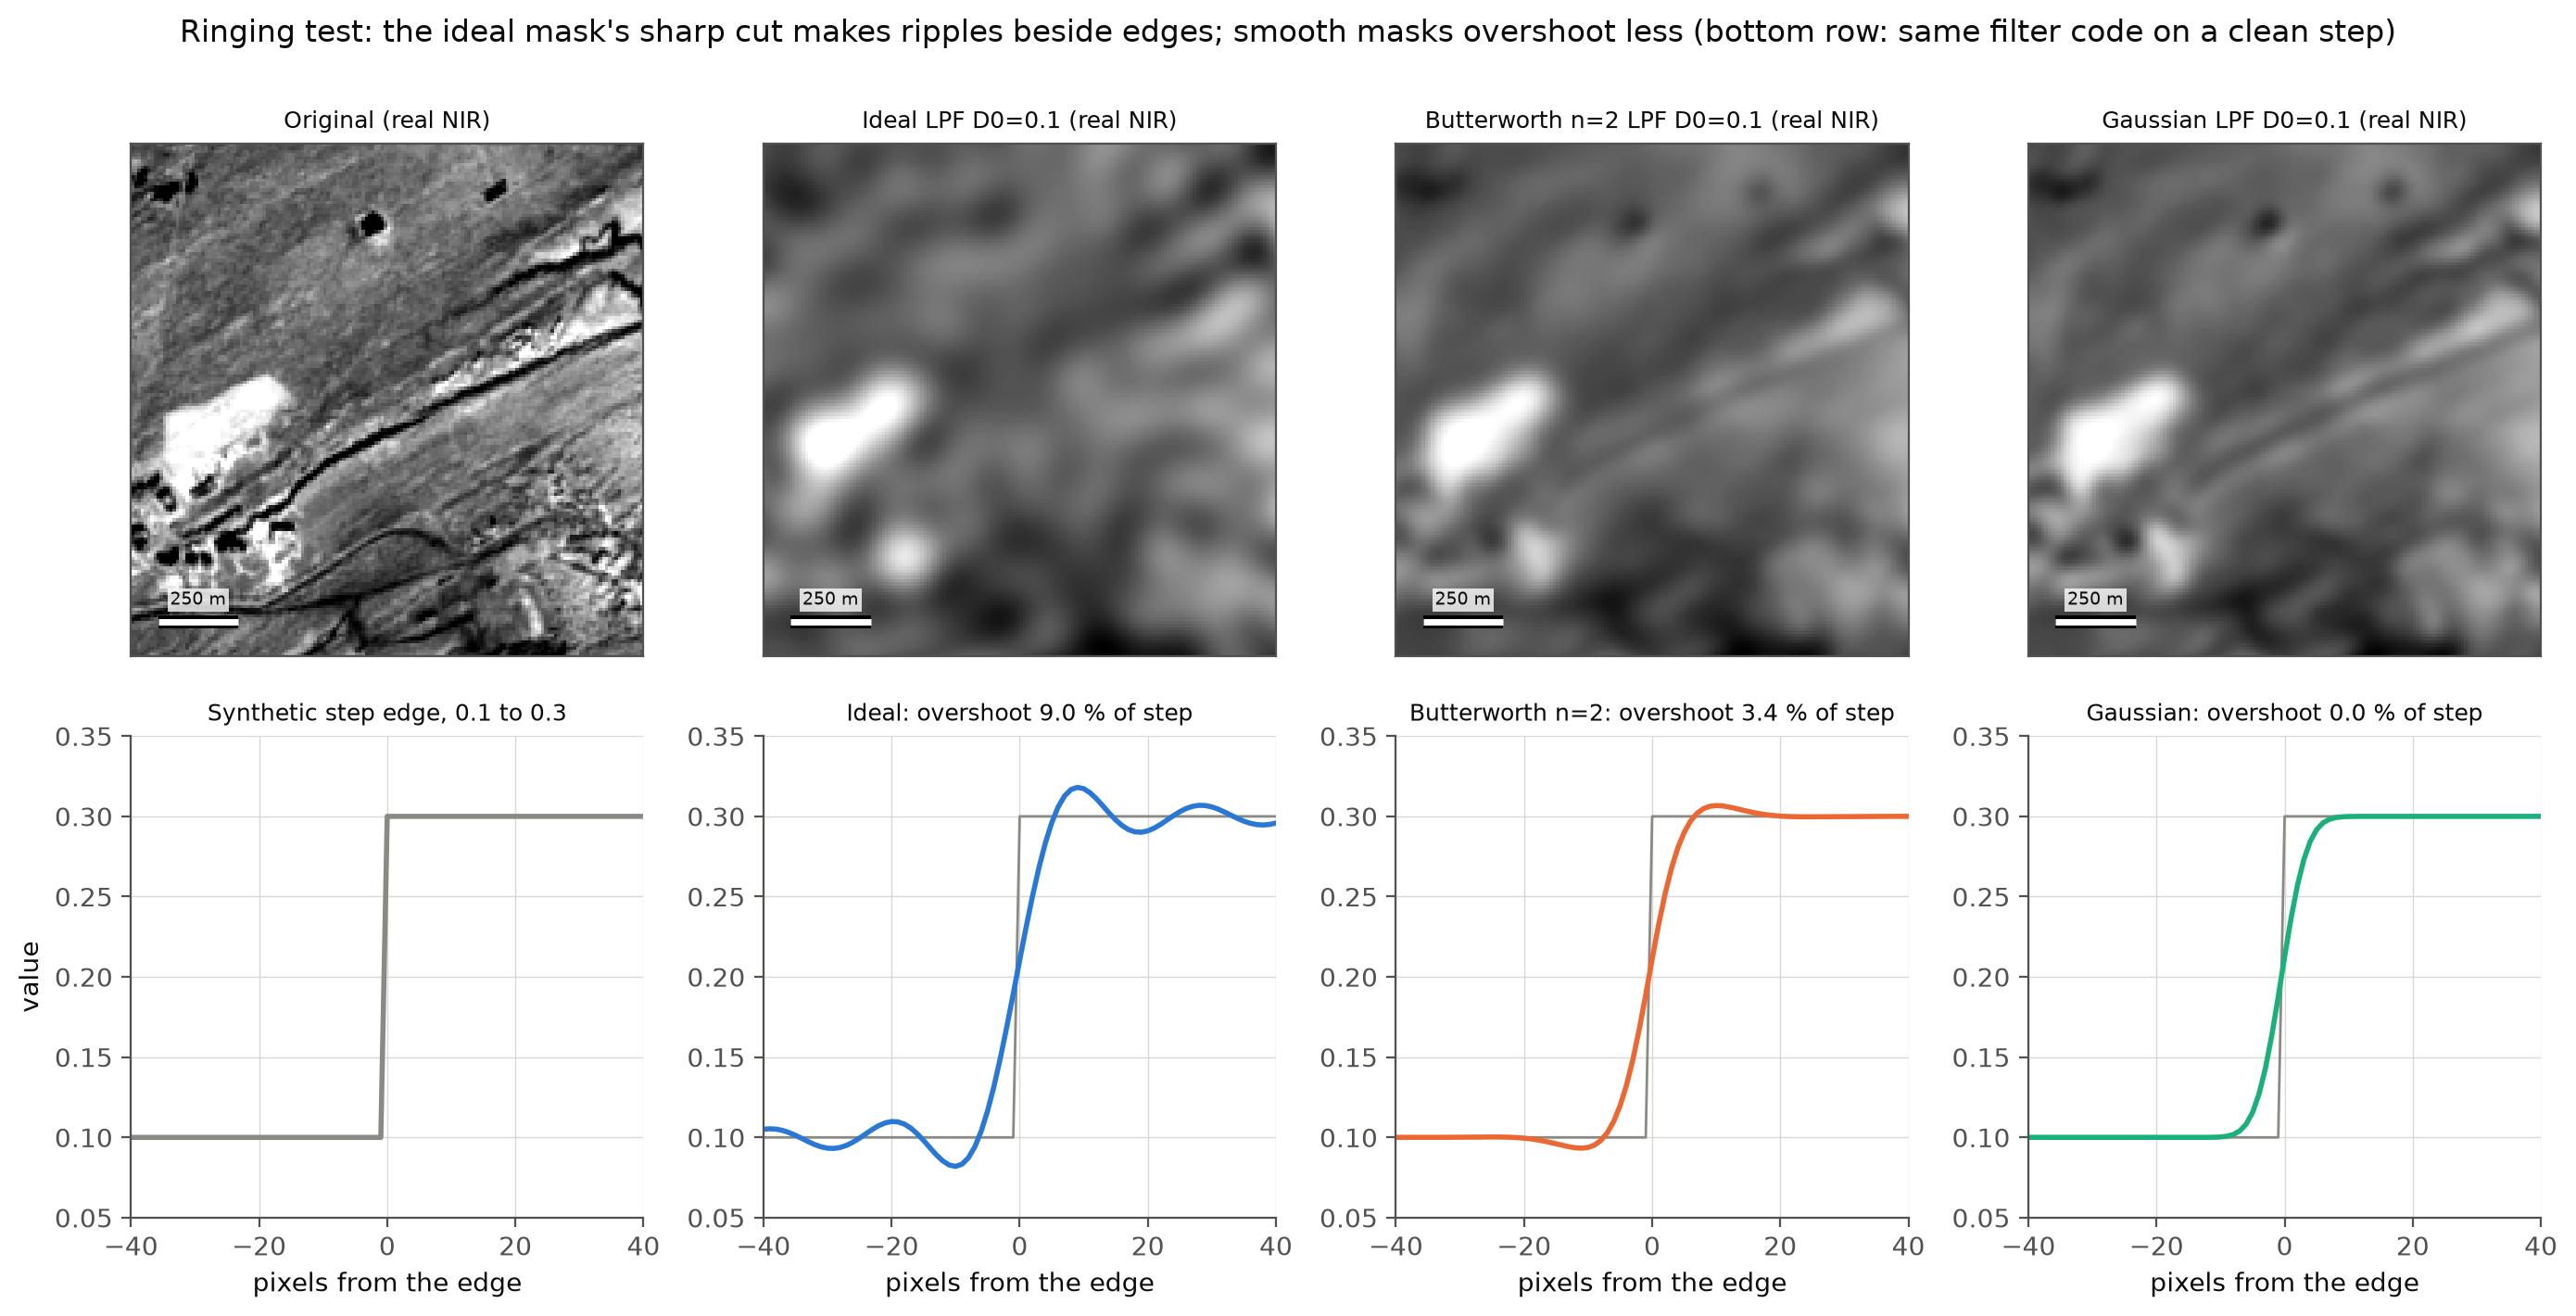
\includegraphics[width=\textwidth]{fig05_ringing.png}
    \caption[Ringing of ideal, Butterworth and Gaussian masks]{Ringing. Top: NIR window after each low-pass mask ($D_0 = 0.1$). Bottom: the same masks applied to a clean step edge.}
    \label{fig:ringing}
\end{figure}

\begin{keypoint}
A sharp cut in frequency always means ripples in space. Use a Gaussian or Butterworth mask, never the ideal one.
\end{keypoint}

\section{E1: Noise removal}

Table~\ref{tab:e1} gives the results for a representative set of filters. With random (Gaussian) noise the noisy image had a PSNR of <<e1_g_noisy>> dB. Only the lightest filters improved on it: <<p:e1_g_best>> reached <<e1_g_best_psnr>> dB, and <<p:e1_g_second>> <<e1_g_second_psnr>> dB. <<e1_g_n_worse>> of the <<e1_g_n_lpf>> low-pass filters made the image worse than doing nothing, because they removed more real detail than noise.

Salt-and-pepper noise behaved very differently. The 3 $\times$ 3 median raised PSNR from <<e1_sp_noisy>> dB to <<e1_sp_best_psnr>> dB, <<e1_sp_gap>> dB ahead of the best linear filter (<<p:e1_sp_lin>>). A mean or Gaussian spreads each spike over its neighbours; the median simply discards it.

\begin{table}[htbp]
\centering
\caption[E1: noise removal]{E1: noise removal on the 512 $\times$ 512 crop. Best value per column in bold. Full results: \texttt{e1\_noise.csv}.}
\label{tab:e1}
\small
\begin{tabular}{@{}lcccc@{}}
\toprule
 & \multicolumn{2}{c}{Gaussian noise, $\sigma=0.02$} & \multicolumn{2}{c}{Salt-and-pepper, 2\%} \\
\cmidrule(lr){2-3}\cmidrule(l){4-5}
Filter & PSNR (dB) & SSIM & PSNR (dB) & SSIM \\
\midrule
<<e1_table>>
\bottomrule
\end{tabular}
\end{table}

\begin{keypoint}
Median $3\times3$ for impulse noise; a light Gaussian ($\sigma = 1$) or $3\times3$ mean for random noise. Larger kernels do more harm than good.
\end{keypoint}

\section{E2: Land-cover classification}

On raw bands the Random Forest reached an overall accuracy of <<e2_raw_oa>> and $\kappa =$ <<e2_raw_kappa>> on the held-out blocks (Table~\ref{tab:e2}). <<e2_lpf_phrase>> The best input was the <<p:e2_best>> (accuracy <<e2_best_oa>>, $\kappa =$ <<e2_best_kappa>>), almost tied with the spatial <<p:e2_second>> ($\kappa =$ <<e2_second_kappa>>). This tie is expected: the two are nearly the same filter, since $\sigma = 1/(\pi \times 0.2) \approx 1.6$ pixels. Smoothing also cleaned up the map: the salt-and-pepper index fell from <<e2_raw_sp>> to <<e2_best_sp>> (Figure~\ref{fig:class}).

High-boost inputs had the opposite effect. The best one (<<p:e2_hb_best>>) reached only $\kappa =$ <<e2_hb_best_kappa>> and the worst <<e2_hb_worst_kappa>>. Adding HPF layers next to the raw bands helped ($\kappa =$ <<e2_stack_best_kappa>>), but less than smoothing.

The reason is that at 10 m a single class contains many different surfaces: roofs of different materials, shadows, mixed pixels at field edges. A pixel-by-pixel classifier is confused by this variation. Smoothing averages it out before the classifier sees it; sharpening makes it larger.

\begin{table}[htbp]
\centering
\caption[E2: land-cover classification]{E2: classification on held-out blocks. Best and worst input of each family; best value per column in bold (lowest for the salt-and-pepper index). Full results: \texttt{e2\_classification.csv}.}
\label{tab:e2}
\small
\begin{tabular}{@{}llcccc@{}}
\toprule
Input & Family & Accuracy & $\kappa$ & Macro-F1 & Salt-and-pepper \\
\midrule
<<e2_table>>
\bottomrule
\end{tabular}
\end{table}

\begin{figure}[htbp]
    \centering
    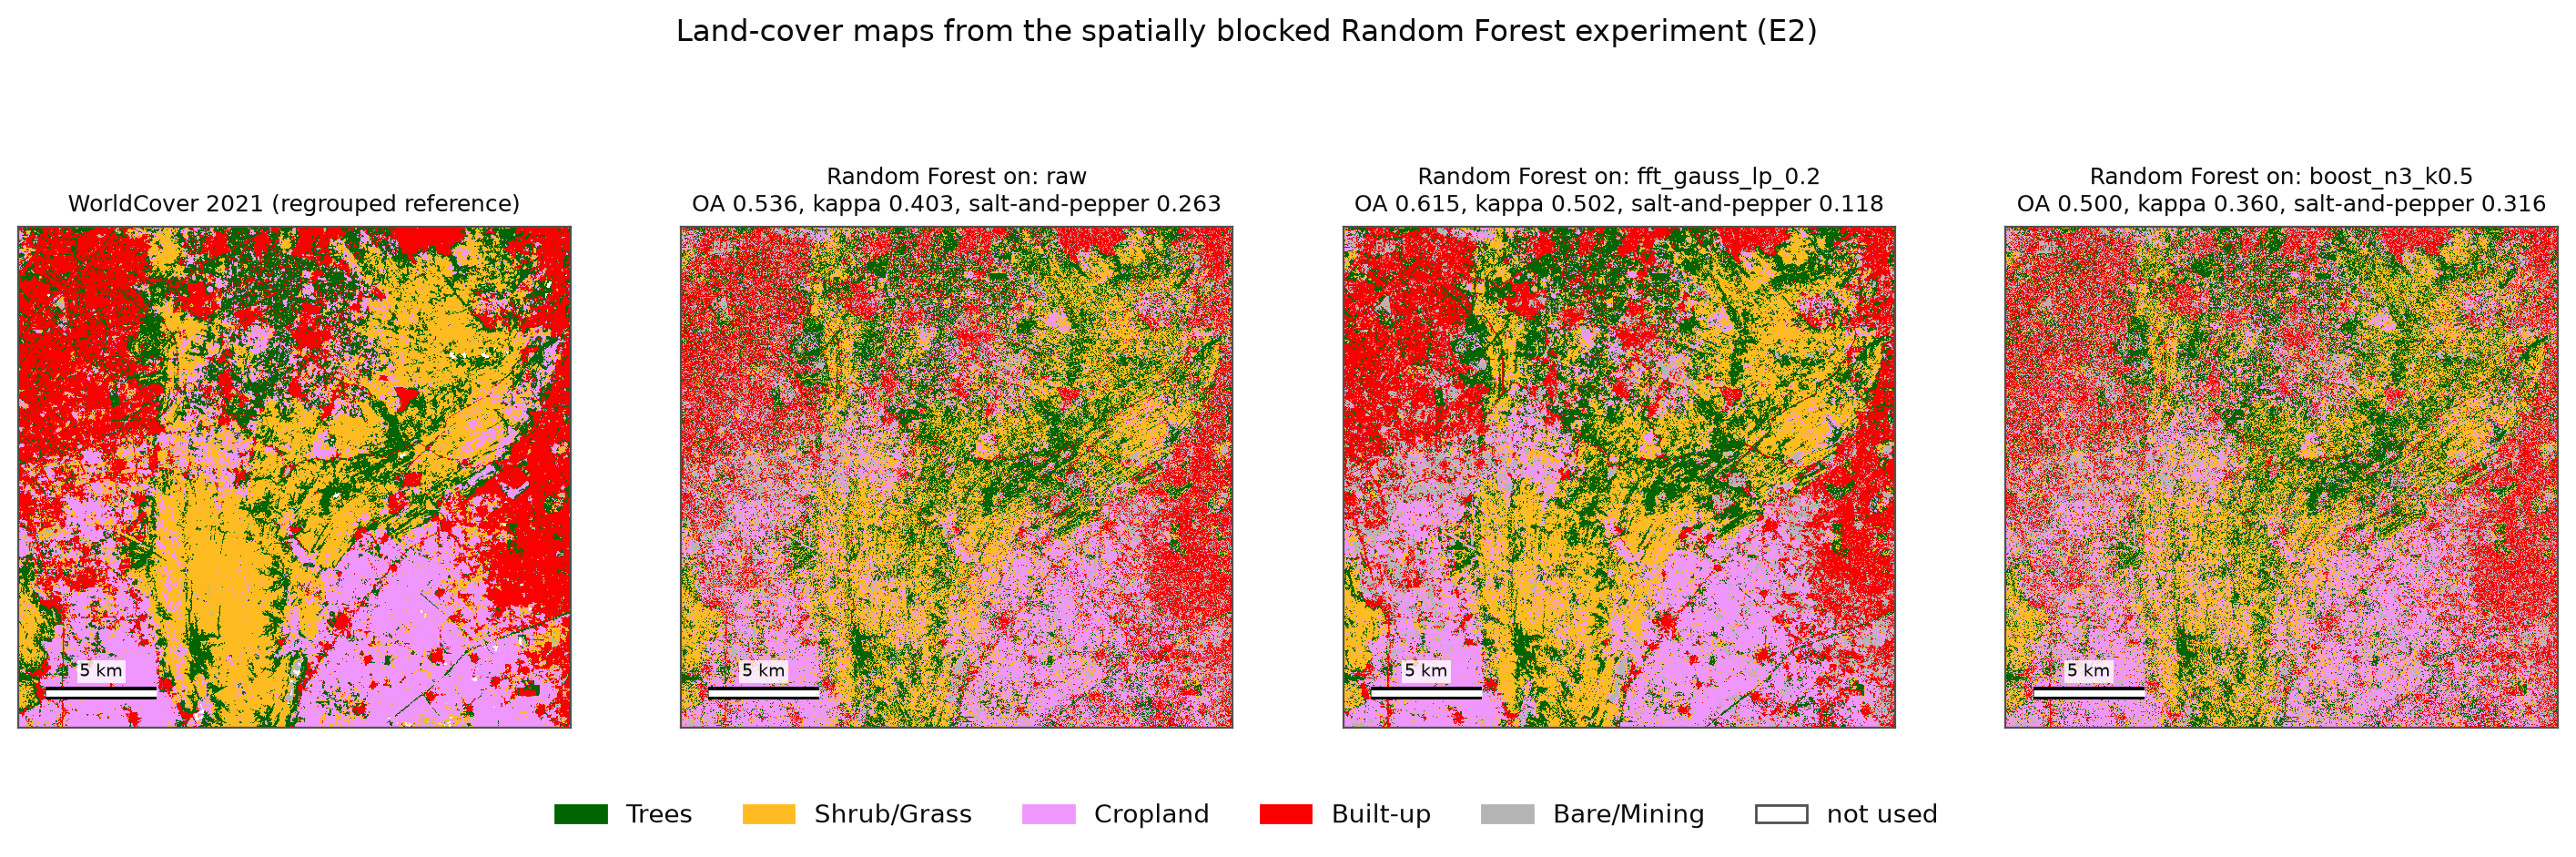
\includegraphics[width=\textwidth]{fig07_classification_maps.png}
    \caption[Classification maps]{WorldCover reference and Random Forest maps from raw bands, the best low-pass input and the best high-boost input.}
    \label{fig:class}
\end{figure}

\begin{keypoint}
For classification, smooth first. A light Gaussian raised $\kappa$ by <<e2_kappa_gain>> and halved map speckle; high-boost lowered $\kappa$.
\end{keypoint}

\section{E3 and E4: Edges, lineaments and spectral change}

Table~\ref{tab:e3e4} puts the edge measures (E3) next to the cost in spectral fidelity (E4) for a set of filters.

\paragraph{Boundaries.} Canny edges from the original NIR band matched WorldCover class boundaries with F1 = <<e3_orig_f1>>. High-boost raised this to <<e3_hb_best_f1>> (<<p:e3_hb_best>>); low-pass filters lowered it (<<e3_box5_f1>> for the 5 $\times$ 5 mean), because fewer edges survive smoothing. For built-up boundaries alone the gain was negligible (<<e3_bu_best_f1>> for <<p:e3_bu_best>> against <<e3_bu_orig>>).

\paragraph{Lineaments.} On the ridge, the original image had a coherence of <<e3_coh_orig>>. Among high-pass outputs only the gradient operators clearly raised it (Prewitt <<e3_coh_prewitt>>, Sobel <<e3_coh_sobel>>). The Laplacian scored lowest (<<e3_coh_lap4>>): it responds to the finest texture, which on the ridge is rock and scrub speckle with no common direction. Low-pass outputs scored even higher (<<e3_coh_g3>> for Gaussian $\sigma = 3$), but only because they erase that speckle along with fine detail; they do not show the lineaments more clearly.

\paragraph{Spectral change.} Light low-pass filters changed the spectra little: a spectral angle of <<e4_med3_sam>>$^\circ$ for the 3 $\times$ 3 median and <<e4_g1_sam>>$^\circ$ for Gaussian $\sigma = 1$. Mild high-boost ($n = 3$, $k = 0.5$) changed them even less (<<e4_hb05_sam>>$^\circ$). Pure HPF outputs are not reflectance any more: their mean is near zero, the spectral angle to the original is about <<e4_hpf_sam>>$^\circ$, and an NDVI computed from them has no meaning.

\begin{table}[htbp]
\centering
\caption[E3 and E4: edges, lineaments and spectral change]{E3 and E4 for selected filters on the NIR band. Edge F1 values are only defined for outputs that are still images. SAM: mean spectral angle to the original; $\Delta$NDVI: mean absolute change in NDVI. Full results: \texttt{e3\_edges.csv}, \texttt{e4\_fidelity.csv}.}
\label{tab:e3e4}
\footnotesize
\setlength{\tabcolsep}{4pt}
\begin{tabular}{@{}lcccccc@{}}
\toprule
 & Mean & Boundary & Built-up & Ridge & SAM & \\
Filter & gradient & F1 & F1 & coherence & ($^\circ$) & $\Delta$NDVI \\
\midrule
<<e3e4_table>>
\bottomrule
\end{tabular}
\end{table}

\begin{keypoint}
High-pass filtering helps wherever the task is about \emph{where things change}: boundaries, ridges, visual sharpness. Keep HPF outputs as separate layers; they cannot replace the bands.
\end{keypoint}

\section{E5: Run time}

On one full <<e5_shape>> band the spatial mean filter took <<e5_box3>> s with a 3 $\times$ 3 kernel and <<e5_box31>> s with 31 $\times$ 31; the spatial Gaussian took <<e5_g8>> s at $\sigma = 8$ (49 $\times$ 49 kernel). Every frequency-domain filter took <<e5_fft_min>>--<<e5_fft_max>> s, whatever the mask or cutoff (Figure~\ref{fig:runtime}). Spatial cost grows with the square of the kernel side; FFT cost does not depend on it. The two cross at a kernel side of about <<e5_cross>> pixels.

\begin{figure}[htbp]
    \centering
    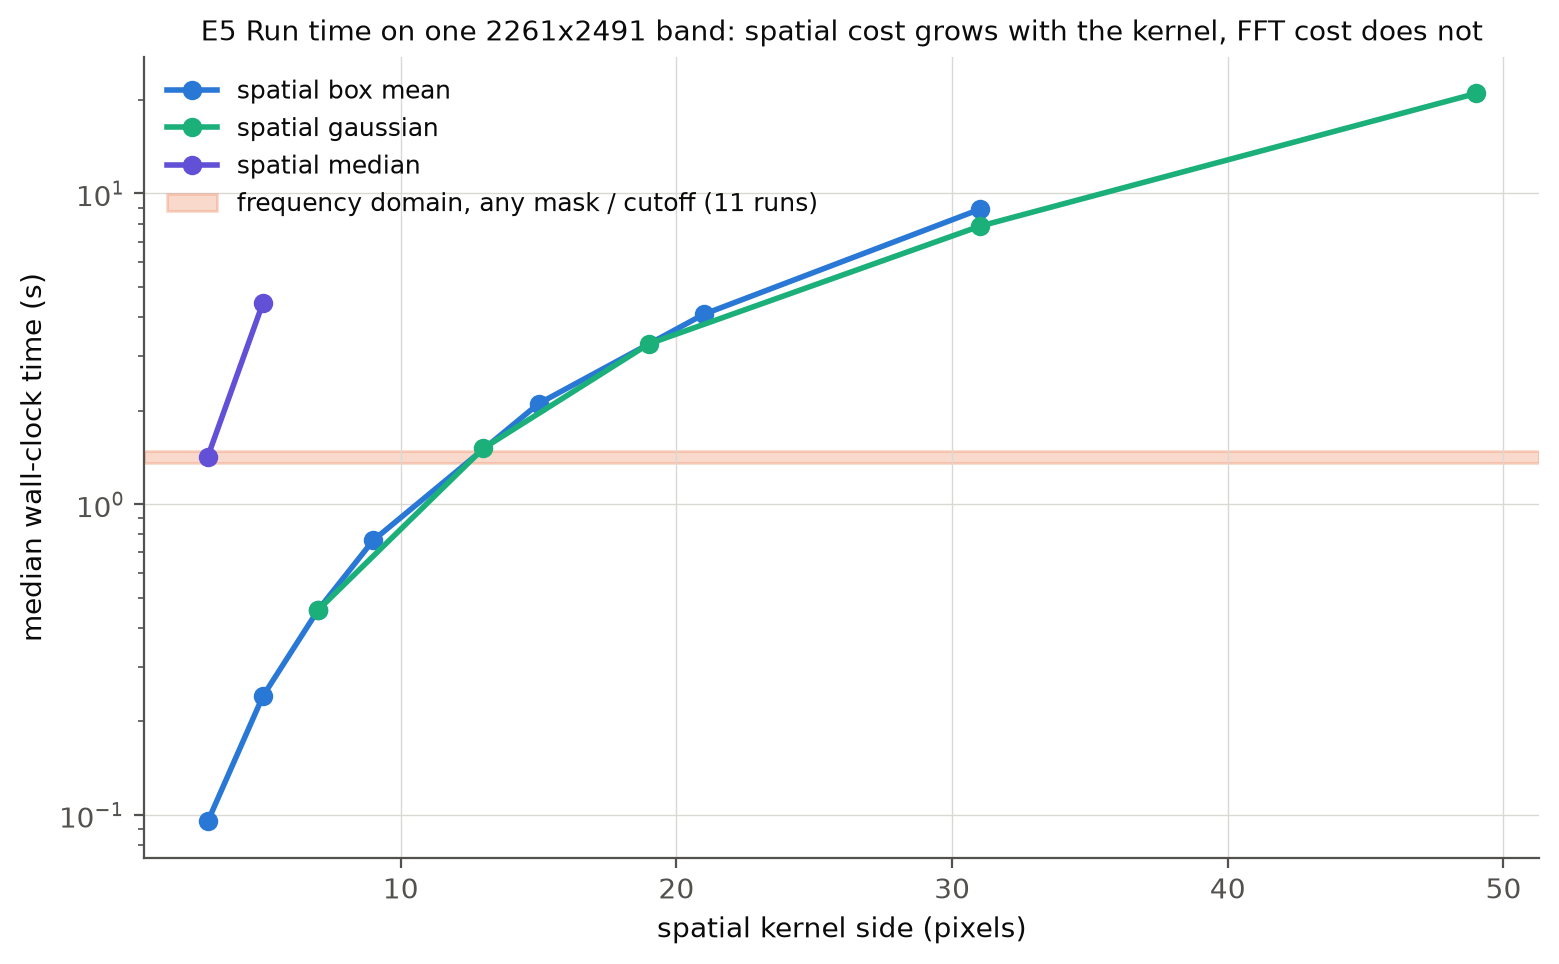
\includegraphics[width=0.85\textwidth]{fig08_e5_runtime.png}
    \caption[Run time of spatial and frequency filtering]{Run time on one full band against kernel size. The shaded band is the range of all frequency-domain runs.}
    \label{fig:runtime}
\end{figure}

% ================================================================ chapter 5
\chapter{Discussion}\label{chap:discussion}

\section{Decision matrix}

Table~\ref{tab:decision} collects the answers. For each application one measure decides the winner, the ``No filter'' column shows what the unfiltered image scores, and the last column gives the cost of the winner as spectral angle. The table is generated by the analysis code (\texttt{decision\_matrix.csv}).

\begin{table}[htbp]
\centering
\caption[Decision matrix]{Decision matrix: best filter for each application.}
\label{tab:decision}
\footnotesize
\setlength{\tabcolsep}{3.5pt}
\begin{tabularx}{\textwidth}{@{}>{\raggedright\arraybackslash}p{2.6cm}>{\raggedright\arraybackslash}p{2.4cm}>{\raggedright\arraybackslash}p{1.9cm}cc>{\raggedright\arraybackslash}Xc@{}}
\toprule
Application & Best filter & Measure & Best & No filter & Runner-up & SAM ($^\circ$) \\
\midrule
<<decision_table_report>>
\bottomrule
\end{tabularx}
\end{table}

\section{When to use which filter}

\paragraph{Low-pass filtering} suits tasks that need clean, stable values per pixel: classification, vegetation indices, change detection. It removed noise and raised classification $\kappa$ by <<e2_kappa_gain>>. The cost is lost boundary detail, and strong smoothing removed real detail faster than noise (E1). Light filters are therefore the right choice.

\paragraph{High-pass filtering} suits tasks about where things change. High-boost with $k$ between 0.5 and 1 gave the best visual sharpening (<<p:vis_best>>: <<vis_gain>> times the original gradient at a spectral angle of <<vis_sam>>$^\circ$) and the best agreement between detected edges and mapped boundaries. For the Aravalli ridges, the Sobel and Prewitt gradient magnitudes brought out the most coherent linear structure. HPF outputs should be stored beside the bands, not instead of them.

\paragraph{Spatial or frequency domain.} With a smooth mask, both routes give the same result (the frequency and spatial Gaussians tie in E2). The frequency route is worth using for large kernels, or when many cutoffs are tried on the same image, because its cost does not grow with the kernel. For the small kernels that work best in practice, convolution is faster and simpler.

\section{Recommendation}

\begin{tcolorbox}[colback=boxbg, colframe=accent, boxrule=0.8pt, arc=2pt, title=\textbf{Which filter for which task}, fonttitle=\small, fontupper=\small]
\begin{itemize}[leftmargin=12pt]
    \item \textbf{Quantitative analysis} (classification, indices, change detection): light low-pass, i.e.\ Gaussian with $\sigma \approx 1.5$--2 pixels, or the frequency Gaussian with $D_0 \approx 0.2$.
    \item \textbf{Impulse noise} (dropped or saturated pixels): 3 $\times$ 3 median.
    \item \textbf{Visual interpretation}: high-boost with $k = 0.5$--1, added on top of the bands.
    \item \textbf{Lineament and structural mapping}: Sobel or Prewitt gradient magnitude as a separate layer.
    \item \textbf{Avoid} the ideal frequency mask for both low-pass and high-pass work because of ringing.
\end{itemize}
\end{tcolorbox}

\section{Limitations}

\begin{itemize}
    \item WorldCover is a model output (ESA reports about 77\% overall accuracy for v200), so E2 and the boundary scores measure agreement with a reference map, not with the ground.
    \item We used one winter scene. Haze, crop stage and soil moisture change through the year, and a second date or a second area would test how general the ranking is.
    \item E2 used one random block split. Differences in $\kappa$ of about 0.01 between the leading filters should not be read as a ranking.
    \item Ridge coherence in one 2 $\times$ 2 km window stands in for lineament quality because no reference lineament map exists for the area.
    \item Bare/Mining covered only <<bare_pct>>\% of the area and was classified poorly by every input (F1 at most <<bare_f1_max>>).
\end{itemize}

% ================================================================ chapter 6
\chapter{Summary}\label{chap:summary}

We implemented low-pass and high-pass filters in both the spatial and the frequency domain and tested <<n_filters>> configurations on a Sentinel-2 scene of the Aravalli ridge. The question ``which is most suitable'' has no single answer, because the two families do opposite jobs. Smoothing helps when pixel values feed a calculation: a light Gaussian gave the most accurate and cleanest land-cover map, and a 3 $\times$ 3 median removed impulse noise. Edge enhancement helps when edges are the point: high-boost gave the sharpest images and best boundary match, and gradient operators gave the clearest ridge lineaments. Among frequency-domain masks, Gaussian and Butterworth are safe while the ideal mask rings. The spatial route is faster for small kernels and the FFT route for kernels of about <<e5_cross>> pixels and more.

% ================================================================ appendix
\appendix

\chapter{Evaluation Measures in Plain Words}\label{app:glossary}

{\small
\begin{xltabular}{\textwidth}{@{}>{\raggedright\arraybackslash}p{3.1cm}X>{\raggedright\arraybackslash}p{2.3cm}@{}}
\caption{What each evaluation measure tells us.}\label{tab:glossary}\\
\toprule
Measure & What it tells us & Better when \\
\midrule
\endfirsthead
\toprule
Measure & What it tells us & Better when \\
\midrule
\endhead
PSNR (dB) & How close the filtered image is to the clean image. It is based on the mean squared error; 3 dB more means about half the error. & higher \\
SSIM & How similar the local patterns (brightness, contrast, structure) are to the clean image, from 0 to 1. & closer to 1 \\
Overall accuracy & Share of test pixels whose class matches WorldCover. & higher \\
Cohen's $\kappa$ & Accuracy after removing the agreement expected by pure chance: 0 is chance level, 1 is perfect. & higher \\
Macro-F1 & F1 score averaged over the classes, so a small class counts as much as a large one. & higher \\
Salt-and-pepper index & Share of map pixels whose class differs from most of their 3 $\times$ 3 neighbours. Measures how speckled a map looks. & lower \\
Boundary F1 & Balance of two shares: detected edges that lie on a mapped class boundary (precision), and mapped boundaries that were detected (recall). A 2-pixel offset is allowed. & higher \\
Average gradient & Mean change in brightness between neighbouring pixels. Measures sharpness. & higher for sharpening \\
Orientation coherence & Whether local edges share one direction (1, parallel ridges) or point every way (0, speckle). & higher for lineaments \\
Spectral angle (SAM) & Angle between a pixel's four-band spectrum before and after filtering. 0$^\circ$ means the shape of the spectrum is unchanged. & lower \\
NDVI change & Mean absolute change in NDVI caused by the filter. & lower \\
Overshoot & How far a filtered step edge rises past its true level, as a percentage of the step height. & lower \\
\bottomrule
\end{xltabular}}

\chapter{Where Each Step Lives in the Code}\label{app:code}

All code is in the Python package \texttt{src/rsfilter/}. Every module and public function has a docstring that explains what it does and why, with formulas where they apply. Table~\ref{tab:code} maps the steps of Figure~\ref{fig:flow} to the code and to the files each step writes.

{\footnotesize
\begin{xltabular}{\textwidth}{@{}>{\raggedright\arraybackslash}p{3.2cm}>{\raggedright\arraybackslash}X>{\raggedright\arraybackslash}p{3.9cm}@{}}
\caption{Map from processing step to code and output.}\label{tab:code}\\
\toprule
Step & Module and main functions & Output \\
\midrule
\endfirsthead
\toprule
Step & Module and main functions & Output \\
\midrule
\endhead
Find and rank scenes, download & \texttt{data.py}: \texttt{fetch\_scene}, \texttt{rank\_candidates} & \texttt{data/raw/}, \texttt{scene\_candidates.csv} \\
Reflectance, WorldCover regrid, sample crop & \texttt{preprocess.py}: \texttt{build\_processed}, \texttt{to\_reflectance}, \texttt{warp\_to\_grid}, \texttt{make\_sample} & \texttt{data/processed/}, \texttt{data/sample/} \\
Spatial filters & \texttt{filters\_spatial.py}: \texttt{convolve2d}, \texttt{mean\_filter}, \texttt{gaussian\_filter}, \texttt{median\_filter}, \texttt{high\_pass}, \texttt{laplacian}, \texttt{sobel}, \texttt{prewitt}, \texttt{high\_boost} & filtered arrays \\
Frequency filters & \texttt{filters\_freq.py}: \texttt{freq\_filter}, \texttt{make\_mask}, \texttt{square\_lowpass}, \texttt{step\_response} & filtered arrays \\
List of all filters & \texttt{bank.py}: \texttt{filter\_bank} & named configurations \\
Classification & \texttt{classify.py}: \texttt{regroup}, \texttt{block\_split}, \texttt{run\_classification} & \texttt{results/maps/} \\
Measures & \texttt{metrics.py}: \texttt{psnr}, \texttt{ssim}, \texttt{boundary\_prf}, \texttt{coherence}, \texttt{spectral\_angle}, \ldots & -- \\
Experiments E1--E5 & \texttt{experiments.py}: \texttt{e1\_noise}, \texttt{e2\_classification}, \texttt{e3\_e4}, \texttt{e5\_runtime}, \texttt{ringing\_table}, \texttt{decision\_matrix} & \texttt{results/tables/*.csv} \\
Figures & \texttt{viz.py} & \texttt{results/figures/} \\
Command line & \texttt{cli.py}: \texttt{fetch}, \texttt{filter}, \texttt{evaluate}, \texttt{figures}, \texttt{demo} & -- \\
Report and slides & \texttt{scripts/build\_latex.py} & \texttt{report/}, \texttt{presentation/} \\
Tests & \texttt{tests/}: our filters against \texttt{scipy.ndimage}, masks, measures & -- \\
\bottomrule
\end{xltabular}}

\chapter{Reproducing the Results}\label{app:repro}

The code, the 512 $\times$ 512 sample data and all result tables are in the project repository. The main commands are:

\begin{table}[H]
\centering
\small
\begin{tabularx}{\textwidth}{@{}>{\ttfamily\raggedright\arraybackslash}p{6.2cm}X@{}}
\toprule
\normalfont Command & What it does \\
\midrule
pip install -r requirements.txt & install the pinned Python packages \\
python -m rsfilter fetch & download the scene and WorldCover (Earth Engine, or open STAC servers as fallback) \\
python scripts/run\_all.py & run E1--E5 and the decision matrix on the full area \\
python scripts/make\_figures.py & redraw all figures \\
python -m rsfilter demo & run the whole pipeline offline on the sample crop in about a minute \\
python -m rsfilter filter ... & apply one filter to a GeoTIFF and keep its georeferencing \\
pytest -q & check every filter against \texttt{scipy.ndimage} \\
python scripts/build\_latex.py & rebuild this report and the slides from the result tables \\
\bottomrule
\end{tabularx}
\end{table}

The algorithm with all formulas, the pseudo-code with array shapes and data types, and a module-by-module code reference are in \texttt{docs/algorithm.md}, \texttt{docs/pseudocode.md} and \texttt{docs/code\_reference.md}.

\clearpage
\phantomsection
\addcontentsline{toc}{chapter}{Bibliography}
\bibliographystyle{plainnat}
\bibliography{references}

\end{document}
